\documentclass[spanish, a4paper, 12pt, final, slideColor, nototal, colorBG, pdf, noaccumulate, darkblue]{beamer}
\usepackage[spanish]{babel}
\usepackage[utf8]{inputenc}
\usepackage{latexsym}
\usepackage{soul}
\usepackage{import}
\usepackage{multicol}
\usepackage{graphicx}
\usepackage{hyperref}
\usepackage{caption}
\usepackage{color}
\usepackage{listings}
\captionsetup{font=scriptsize,labelfont=scriptsize}
\DeclareGraphicsExtensions{.pdf,.png,.jpg}

% Mathematics
\usepackage{amssymb}
\usepackage{amsfonts}
\usepackage{anysize}
\usepackage{float}
\usepackage{amsthm}
\usepackage{amsmath}
\usepackage{verbatim}
\usepackage{mathtools}
\usepackage{tikz}
\usefonttheme[onlymath]{serif}

\providecommand{\abs}[1]{\left\lvert#1\right\rvert}
\providecommand{\norm}[1]{\left\lVert#1\right\rVert}
\providecommand{\norminf}[1]{\norm{#1}_{\infty}}
\providecommand{\bholomorphic}[1]{\mathcal{H}^{\infty}(#1)}

\newcommand*\xbar[1]{%
   \hbox{%
     \vbox{%
       \hrule height 0.5pt % The actual bar
       \kern0.2ex%         % Distance between bar and symbol
       \hbox{%
         \kern-0.1em%      % Shortening on the left side
         \ensuremath{#1}%
         \kern-0.1em%      % Shortening on the right side
       }%
     }%
   }%
}

\newcommand{\complex}{\mathbb{C}}
\newcommand{\disk}{\mathbb{D}}
\newcommand{\closedisk}{\overline{\disk}}
\renewcommand{\Re}{\operatorname{Re}}
\newcommand{\id}{\operatorname{id}}
\newcommand{\fiber}{\mathfrak{M}}

\makeatletter
\newcommand{\leqnomode}{\tagsleft@true}
\newcommand{\reqnomode}{\tagsleft@false}
\makeatother

\newtagform{Alph}[\renewcommand{\theequation}{\Alph{equation}}]()
\newtagform{alph}[\renewcommand{\theequation}{\alph{equation}}]()
\newtagform{Roman}[\renewcommand{\theequation}{\roman{equation}}]()
\newtagform{roman}[\renewcommand{\theequation}{\roman{equation}}]()
\newtagform{scroman}[\renewcommand{\theequation}{\scshape\roman{equation}}][]

\newcounter{align}[equation]
\renewcommand{\thealign}{\roman{align}}
\newcommand{\alignno}{\refstepcounter{align}\tag{\thealign}}
\expandafter\let\expandafter\oldalignstar\csname align*\endcsname
\expandafter\def\csname align*\endcsname{\refstepcounter{equation}\oldalignstar}

\definecolor{lavander}{RGB}{230, 225, 250}
\definecolor{Numbers}{rgb}{0.5,0.5,0.5}
\definecolor{Keywords}{rgb}{0,0,1}
\definecolor{Emph}{rgb}{0.58,0,0.82}
\definecolor{Strings}{rgb}{0,0.6,0}
\definecolor{Comments}{rgb}{0.6,0.6,0.6}
\definecolor{Background}{rgb}{0.98,0.98,0.98}

\lstset{
breaklines=true,
numbers=left,
numberstyle=\tiny\color{Numbers},
numbersep=5pt,
rulecolor=\color{black},
stepnumber=1,
xleftmargin=1em,
framextopmargin=2em,
framexbottommargin=2em,
showspaces=false,
showtabs=false,
showstringspaces=false,
frame=l,
tabsize=2,
% Basic
basicstyle=\scriptsize, %footnotesize
backgroundcolor=\color{Background},
% Comments
commentstyle=\color{darkgray}\slshape,
% Strings
stringstyle=\color{Strings},
morecomment=[s][\color{Strings}]{"""}{"""},
morecomment=[s][\color{Strings}]{'''}{'''},
% keywords
keywordstyle={\color{Keywords}\bfseries},
morekeywords={import,from,class,def,for,while,if,is,in,elif,else,not,and,or,print,break,continue,return,True,False,None,access,as,del,except,exec,finally,global,lambda,pass,print,raise,try,assert},
emph={__init__, self, @staticmethod},
emphstyle=\color{Emph},
% language
language=python
%
}

\usetheme{Madrid}

\title{Problemas geométricos que arrancan de la teoría clásica de funciones}
\author{Celia de Frutos Palacios \thanks{\url{https://github.com/Celia95/TFG}}}
\subtitle{}
\institute[UCM]{}

\logo{
\includegraphics[height=0.7cm]{Imagenes/Vectorial/escudoUCM.png}}

\date{\today}

\begin{document}
\maketitle

\begin{frame}
    \frametitle{Objetivos}
    \begin{itemize}
        \item Estudiar el comportamiento de funciones en el disco unidad.
        \item Analizar cuándo una función puede extenderse a la frontera.
        \item Mostrar la interacción entre los valores en la frontera y el interior del disco.
        \item Desarrollar aplicaciones informáticas que permitan visualizar y analizar ejemplos concretos.
    \end{itemize}
\end{frame}

\begin{frame}
    \frametitle{Antecedentes}
    \begin{itemize}
        \item Cauchy: uso de integración en el estudio de funciones holomorfas.
        \item Riemann: punto de vista geométrico y funciones conformes.
        \item Weierstrass: series de potencias y productos infinitos.
    \end{itemize}
    En el desarrollo del trabajo nos adentramos en cuestiones que desarrollan aspectos de nuestro problema desde los tres puntos de vista: analítico, geométrico y algebraico.
\end{frame}

\begin{frame}
    \frametitle{Problema de Dirichlet}
    \begin{block}{}
        Dada una función $f: \partial \disk \to \complex$ continua queremos encontrar una función armónica en el disco que coincide en el borde del disco con $f$.
    \end{block}
\end{frame}


\begin{frame}
    \frametitle{Integral de Poisson}
    \begin{itemize}
        \item Integral de Poisson de una función $f \in L^1(\partial \disk)$:
            \begin{equation*}
                F = P[f]: z=re^{i \theta} \in \disk \mapsto F(re^{i \theta}) = \dfrac{1}{2 \pi} \int_{- \pi}^{\pi} P_r (\theta - t) f(e^{it}) dt.
            \end{equation*}

        \item La integral de Poisson proporciona una solución afirmativa al problema de Dirichlet.
            \begin{equation*}
                u : z = re^{i \theta} \in \closedisk \mapsto u(re^{i \theta}) =
                \begin{cases}
                    f(e^{i\theta}) & \text{si } r=1 \\
                    F(re^{i\theta}) & \text{si } 0 \leq r<1
                \end{cases}
            \end{equation*}
    \end{itemize}
\end{frame}

\begin{frame}
    \frametitle{Teorema de Fatou y teorema de Carathéodory}
    \begin{block}{Teorema de Fatou}
         Para toda función $f \in \bholomorphic{\disk}$, existe una función $f^* \in L^{\infty} (\partial \disk)$ definida por
         \begin{equation*}
            f^*(e^{it}) = \lim_{r \to 1} f(re^{it})
        \end{equation*}
        en casi todo punto.
    \end{block}

    \begin{block}{Teorema de Carathéodory}
        Sea $\varphi$ una aplicación conforme del disco unidad $\disk$ en un dominio de Jordan $\Omega$. Entonces $\varphi$ tiene una extensión continua al disco cerrado $\closedisk$, y la extensión es inyectiva de $\closedisk$ en $\xbar{\Omega}$.
    \end{block}

\end{frame}

\begin{frame}
    \frametitle{Representación de $e^{\frac{z-i}{z+i}}$ y límites radiales}
    \begin{figure}[!htbp]
        \centering
        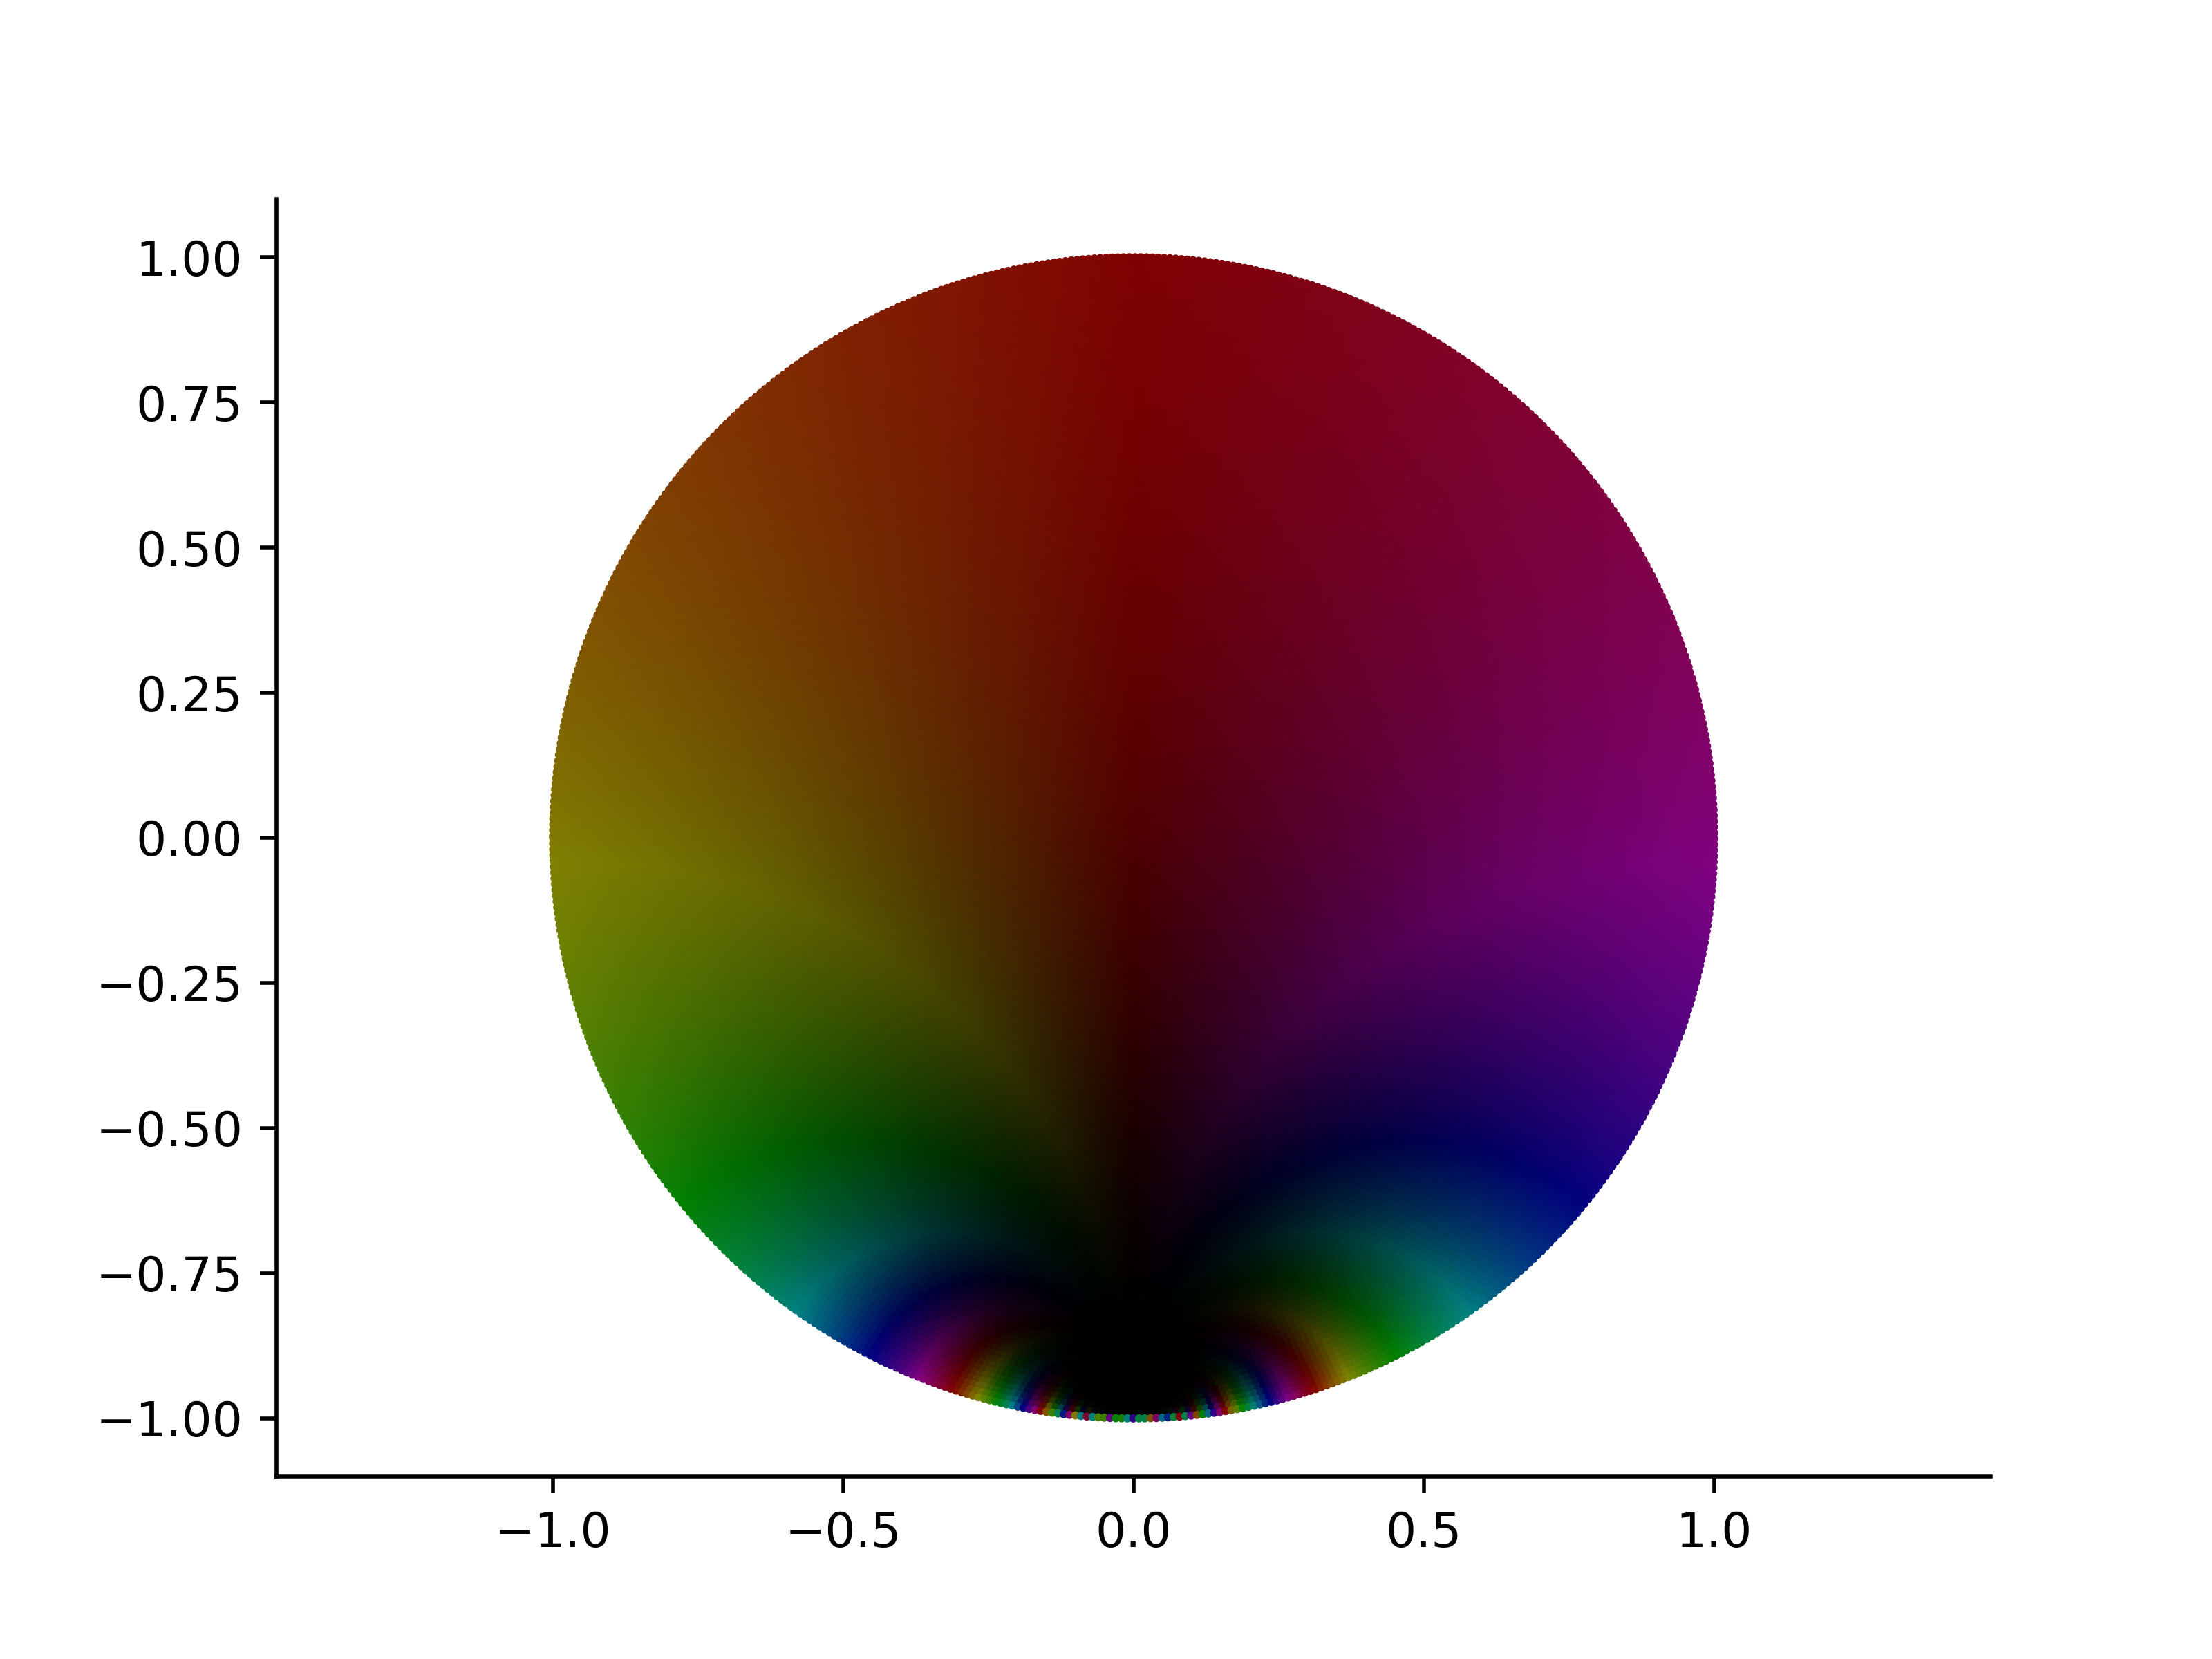
\includegraphics[width=0.7\textwidth]{../Aplicacion/e^((z-i):(z+i)).png}
        \label{fig:e^((z-i)/(z+i))}
    \end{figure}
\end{frame}

\begin{frame}
    \frametitle{Aplicación informática}
    \begin{itemize}
        \item Técnica de coloreado del dominio (\textit{domain coloring}).
        \item Representación de funciones complejas.
        \item Resolución del problema de Dirichlet para el disco.
    \end{itemize}
\end{frame}

\begin{frame}
    \frametitle{Técnica de coloreado del dominio}
    \begin{figure}[!htbp]
        \centering
        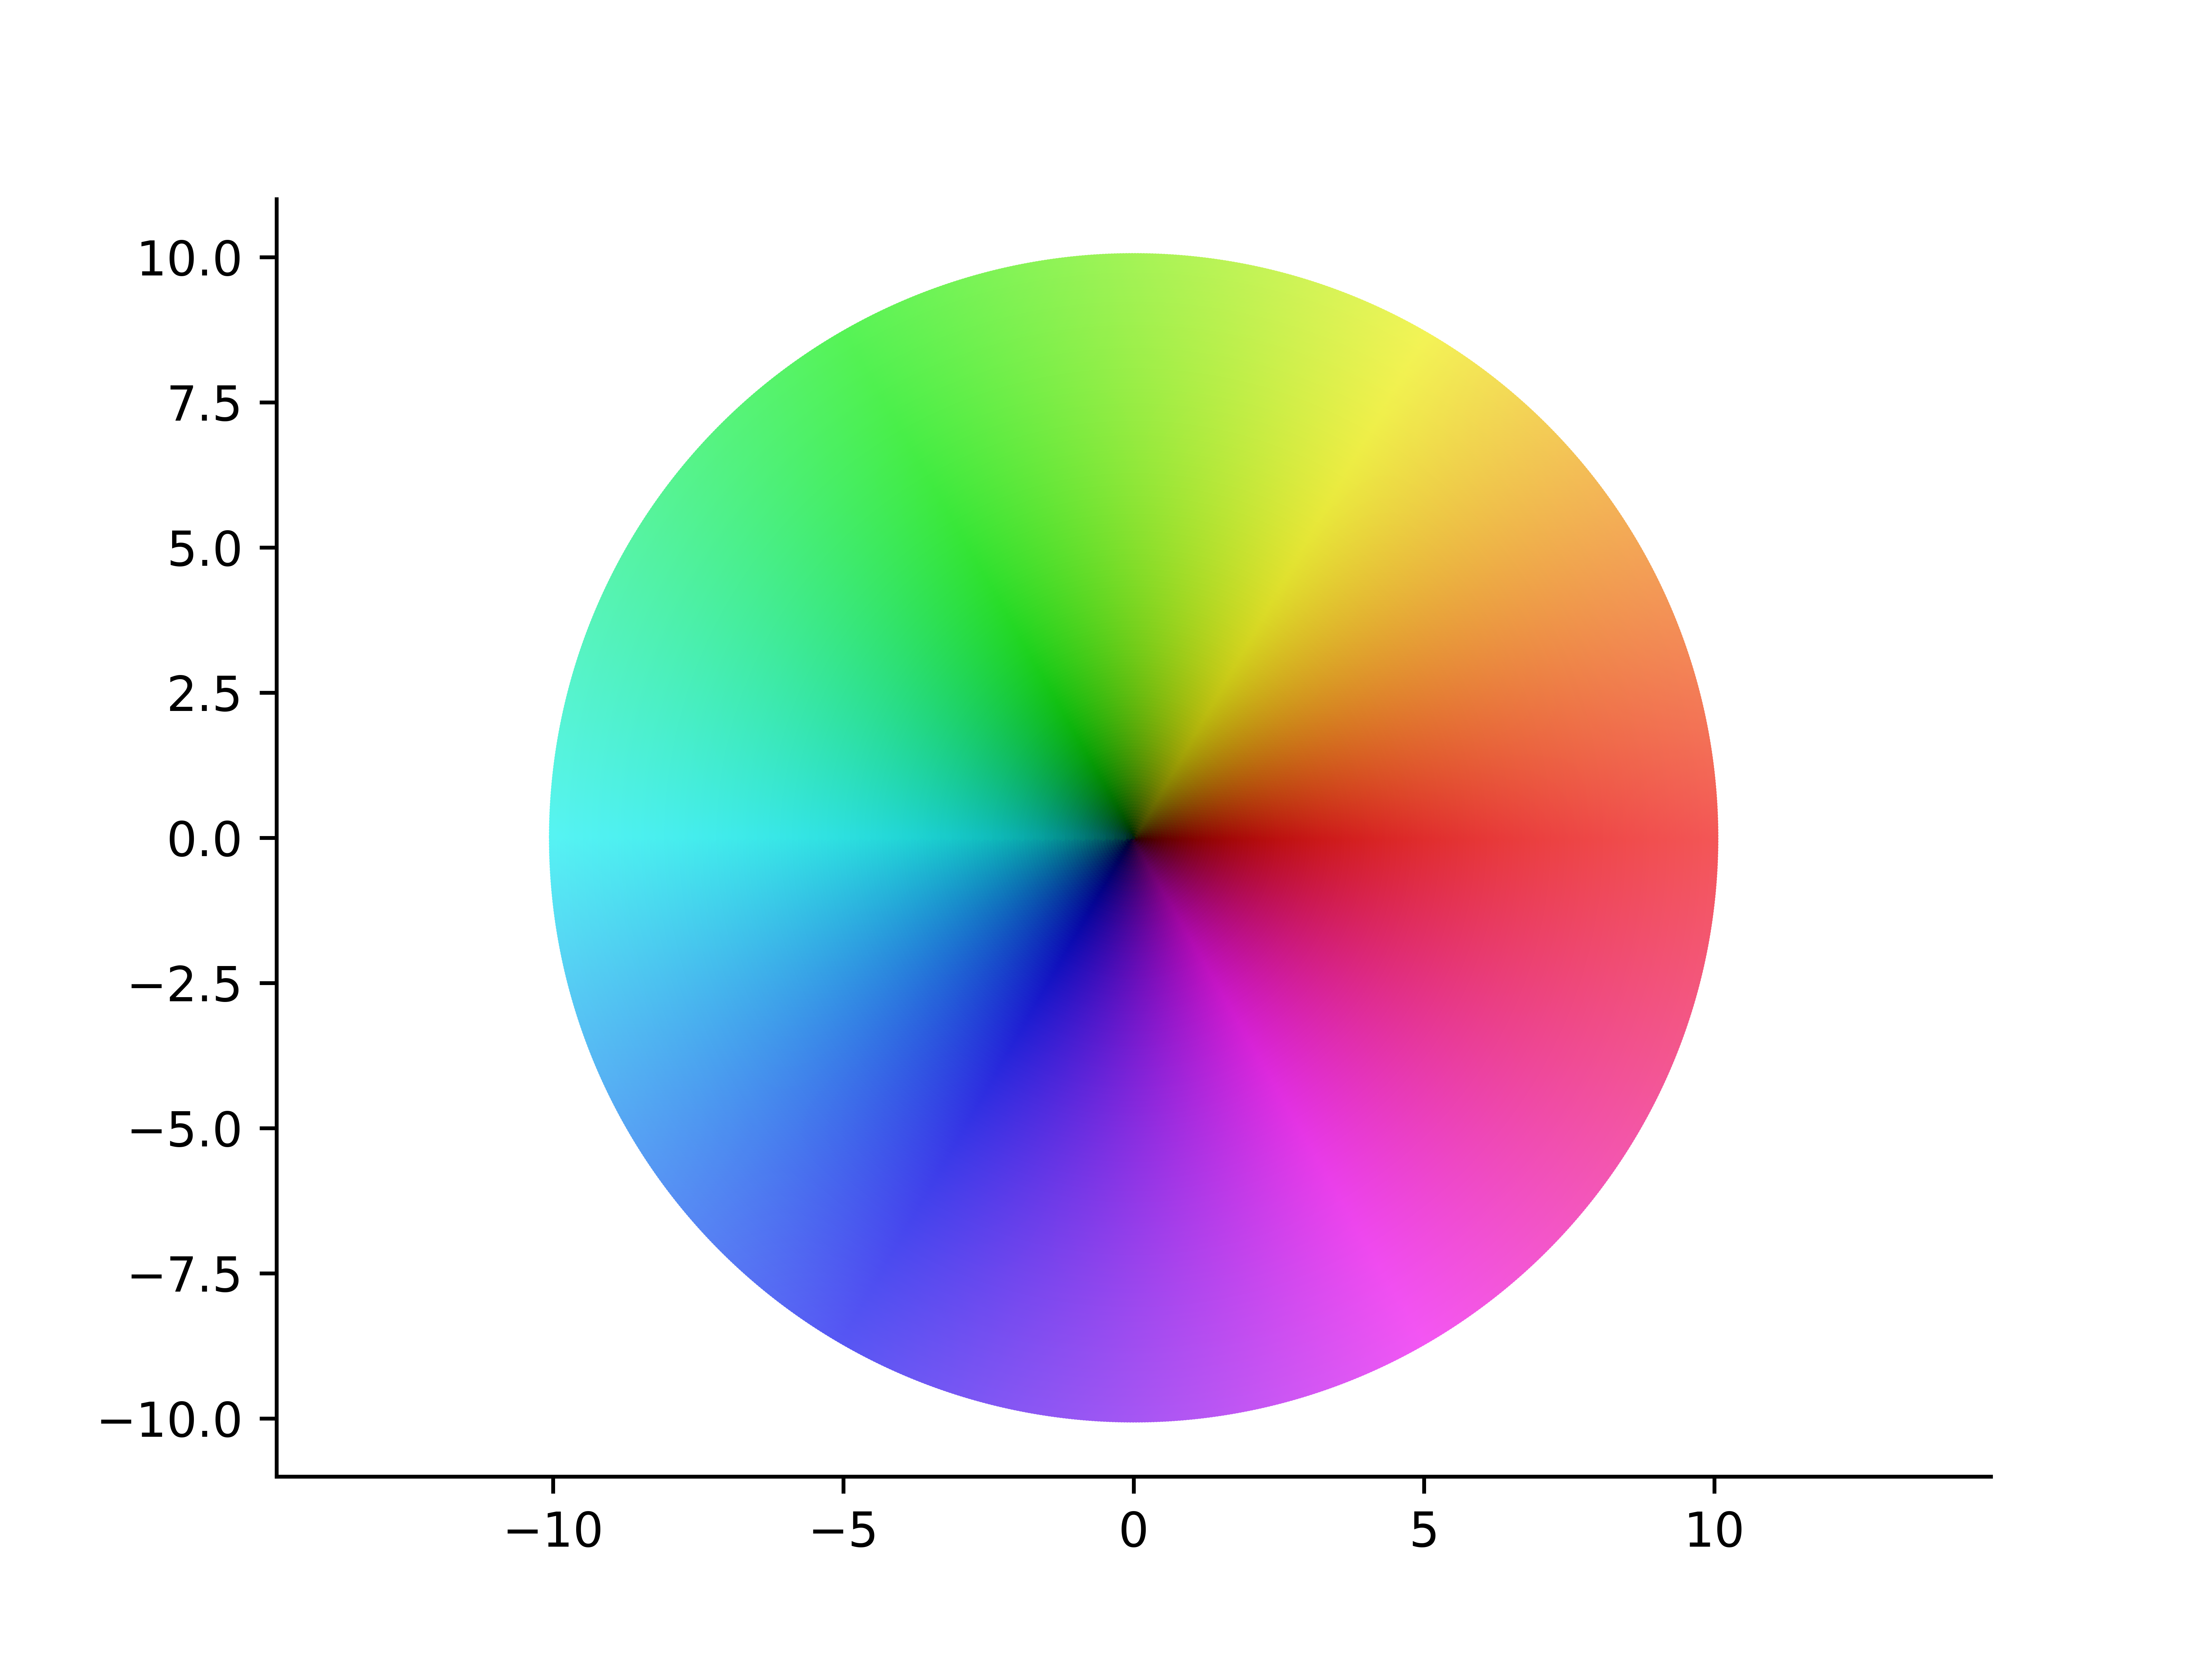
\includegraphics[width=0.7\textwidth]{../Aplicacion/z.png}
        \label{fig:z}
    \end{figure}
\end{frame}

\begin{frame}
    \frametitle{Representación de $z^3$}
    \begin{figure}[!htbp]
        \centering
        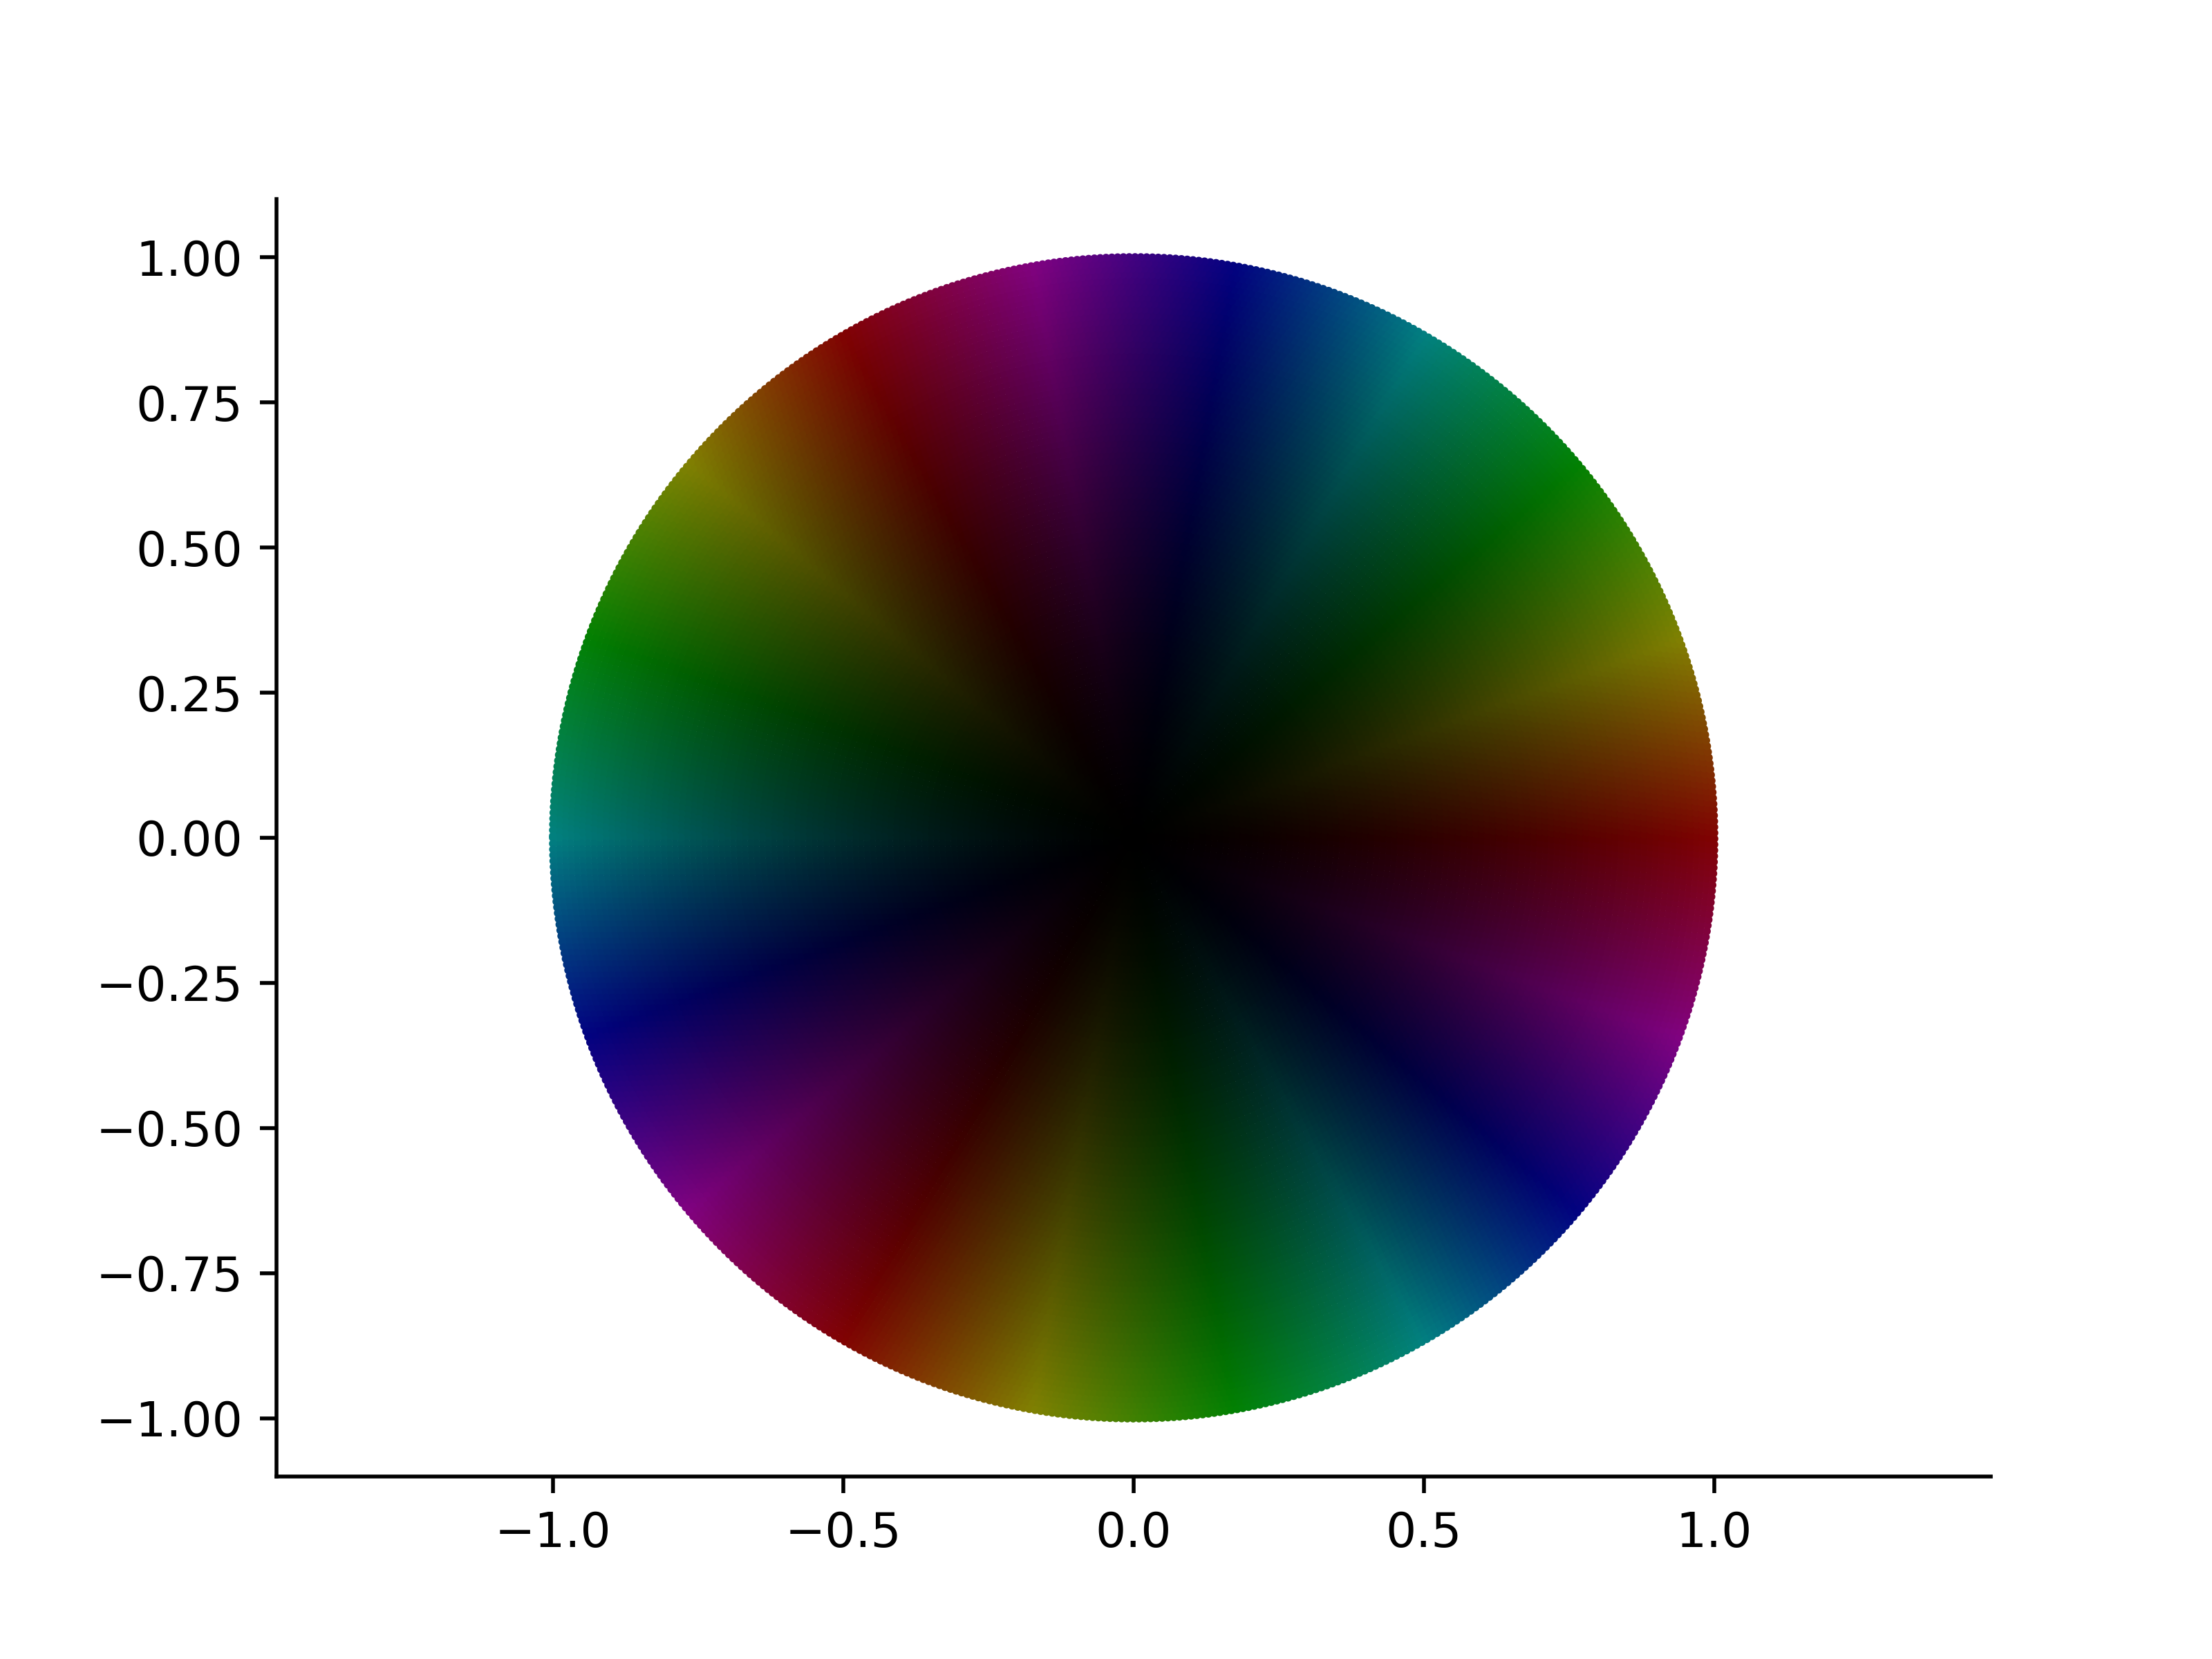
\includegraphics[width=0.7\textwidth]{../Aplicacion/z^3(2).png}
        \label{fig:z^3(2)}
    \end{figure}
\end{frame}

\begin{frame}
    \frametitle{Representación de $e^{z^3}-1$}
    \begin{figure}[!htbp]
        \centering
        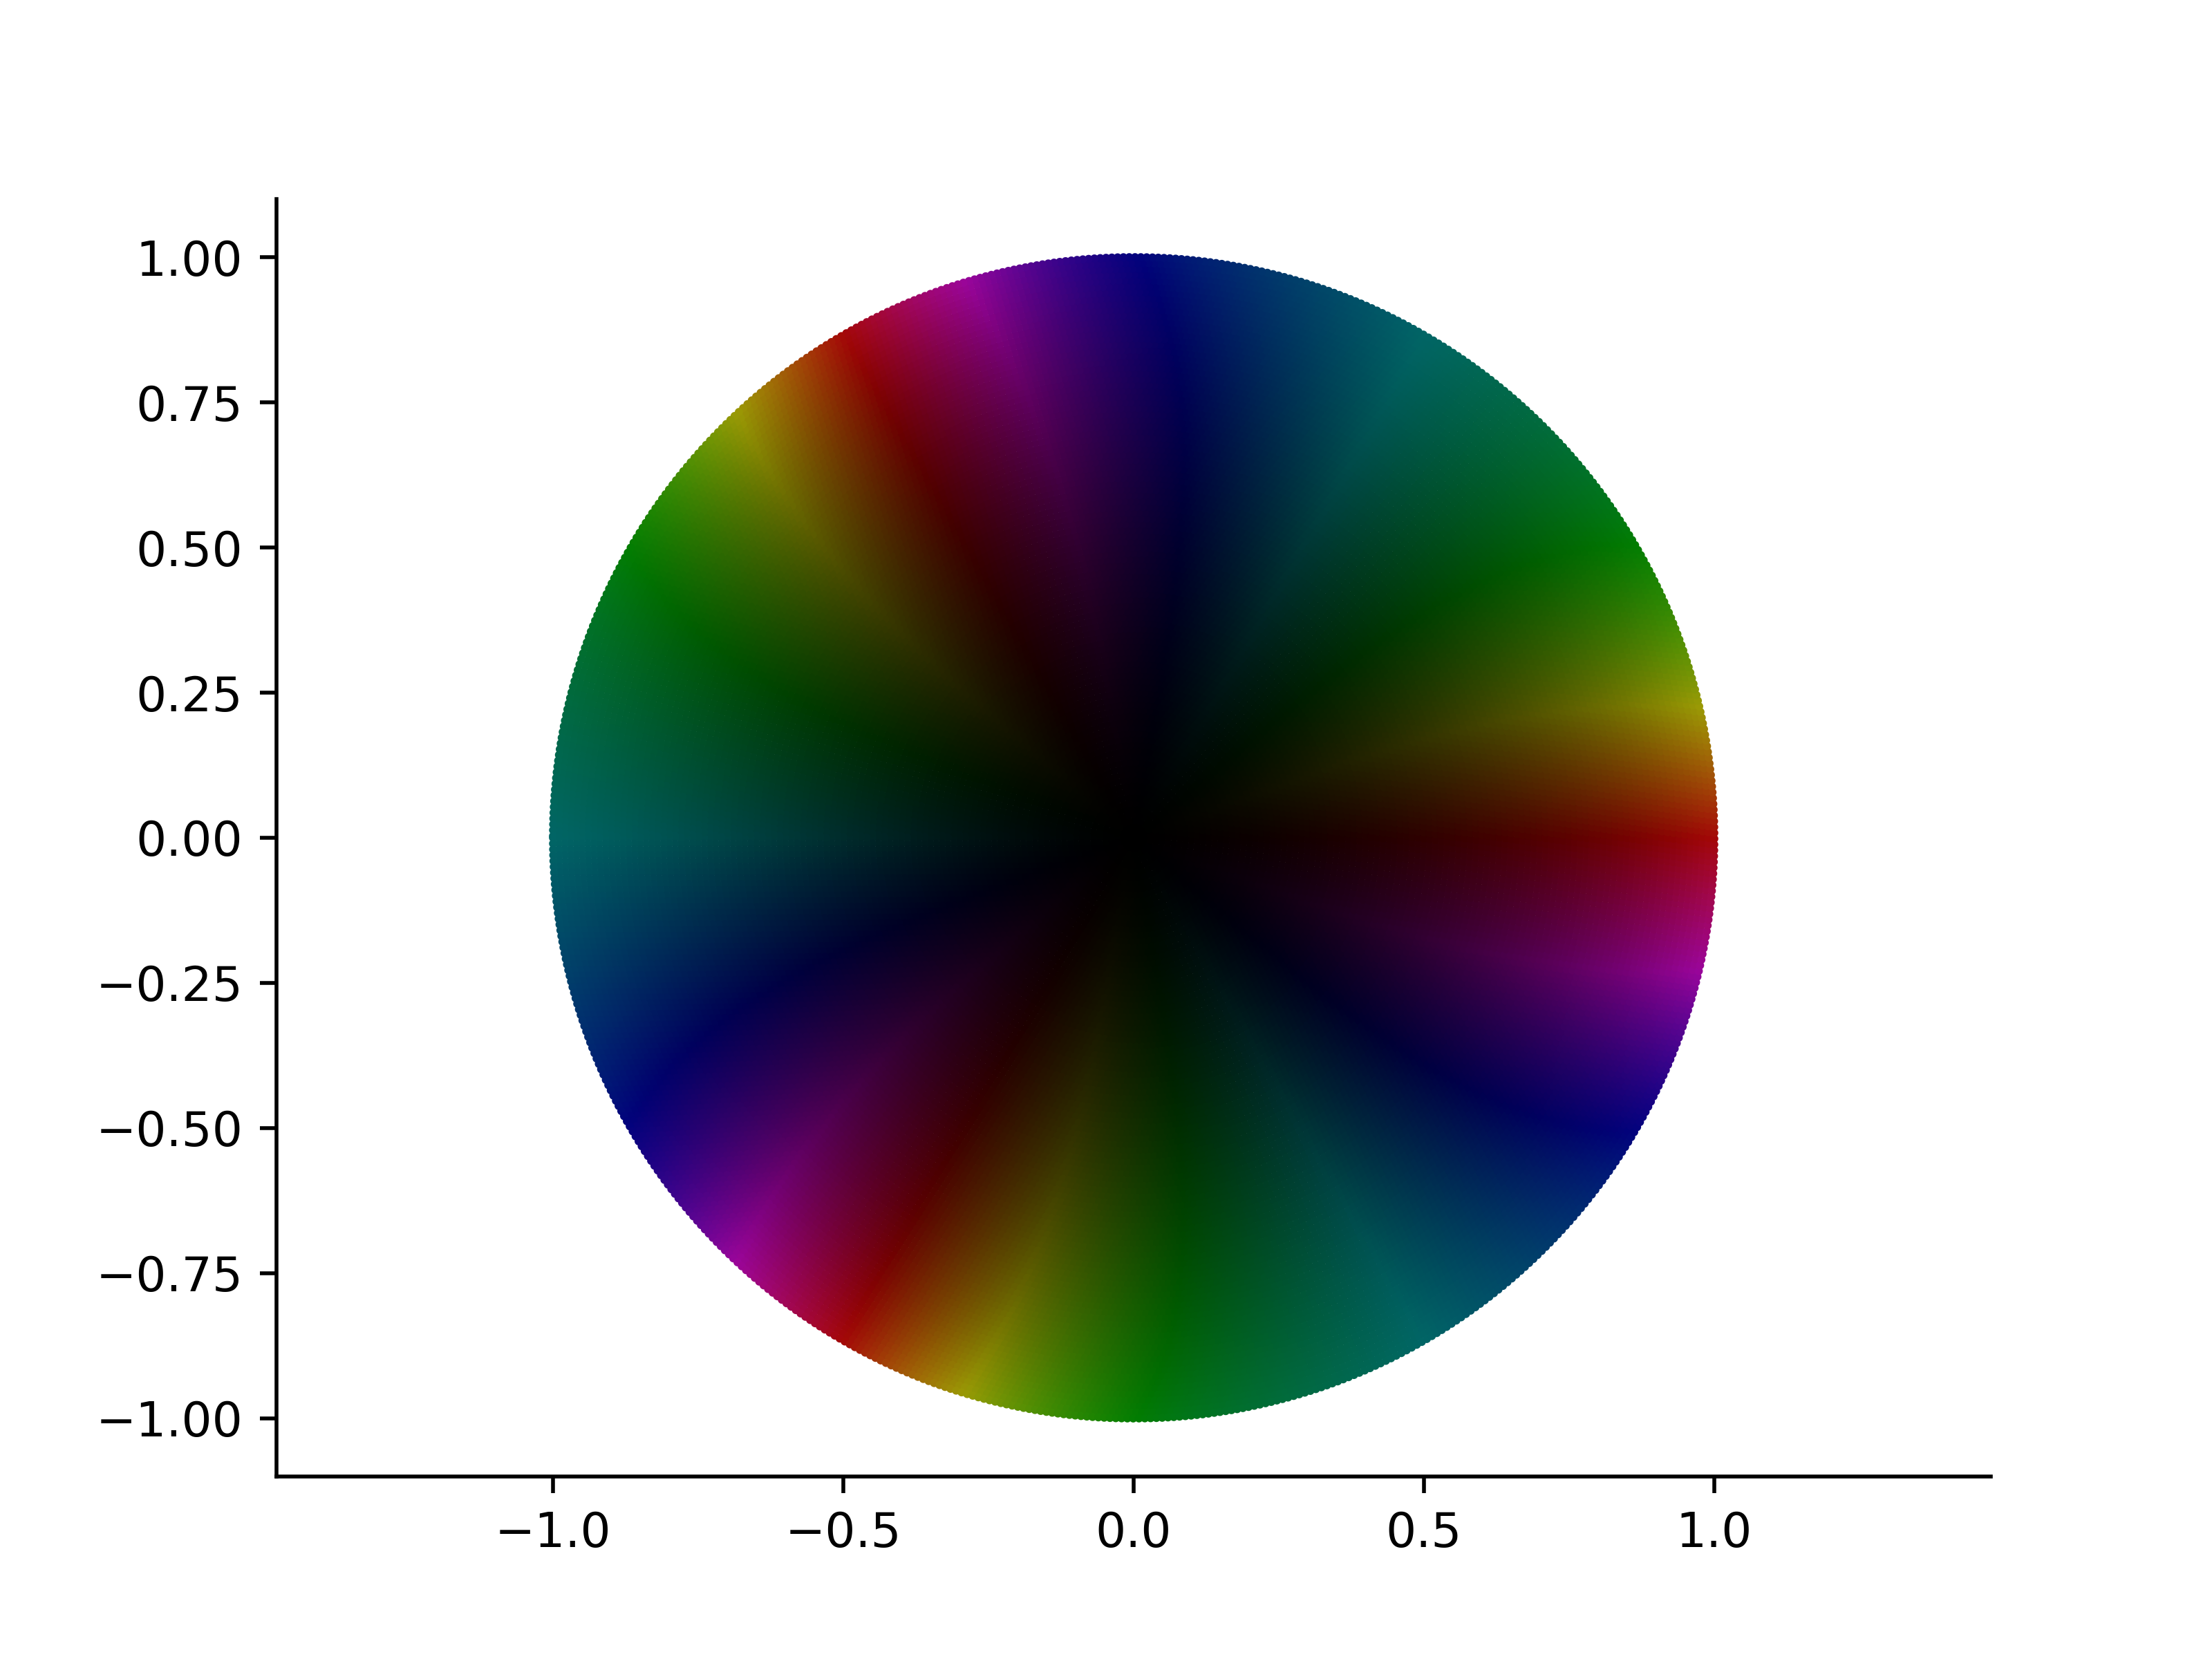
\includegraphics[width=0.7\textwidth]{../Aplicacion/e^(z^3)-1.png}
        \label{fig:e^(z^3)-1}
    \end{figure}
    \begin{equation*}
        e^{z^3} - 1 = z^3 + \frac{z^6}{2!} + \frac{z^9}{3!} + \cdots
    \end{equation*}
\end{frame}


\begin{frame}
    \frametitle{Diferencia entre $z^3$ y $e^{z^3}-1$}
    \begin{figure}[!htbp]
        \centering
        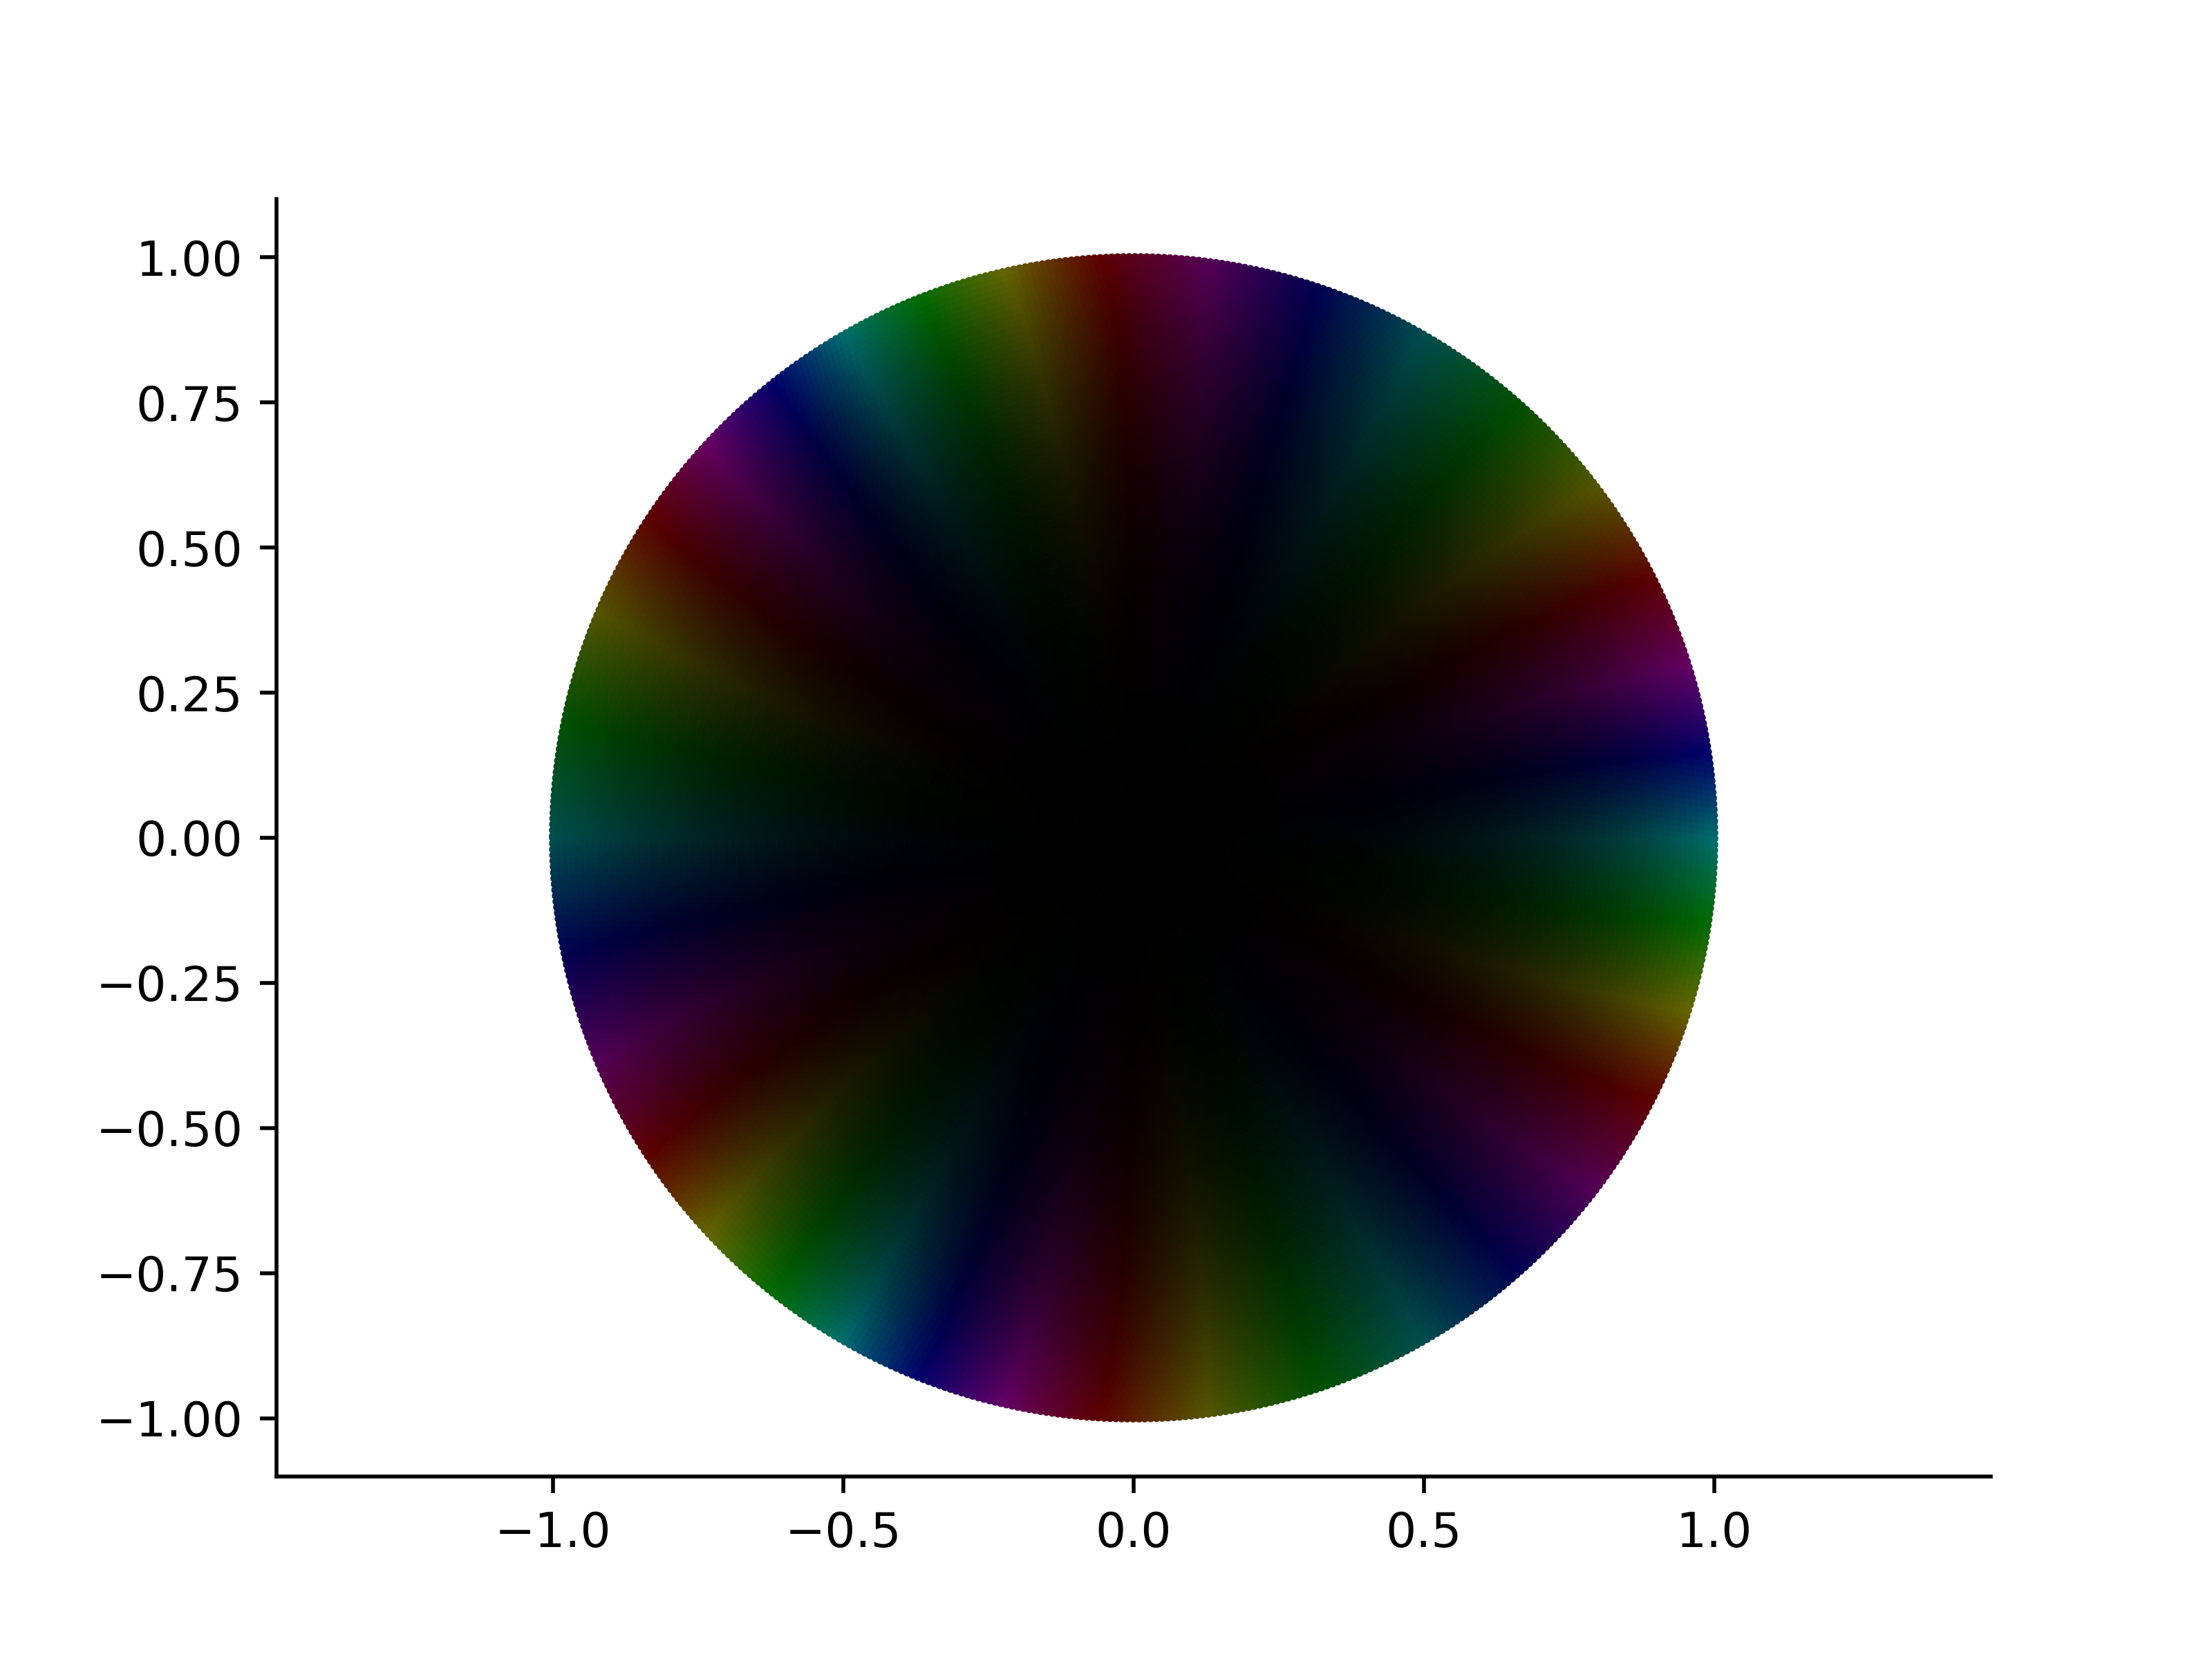
\includegraphics[width=0.7\textwidth]{../Aplicacion/diff6.png}
        \label{fig:diff6}
    \end{figure}
    \begin{equation*}
        e^{z^3} - 1 - z^3 = \frac{z^6}{2!} + \frac{z^9}{3!} + \frac{z^{12}}{4!} + \cdots
    \end{equation*}

\end{frame}

\begin{frame}
    \frametitle{Extensión al disco de la función $e^{10 \cos(t)+10i \sen(t)}$}
    \begin{figure}[!htbp]
        \centering
        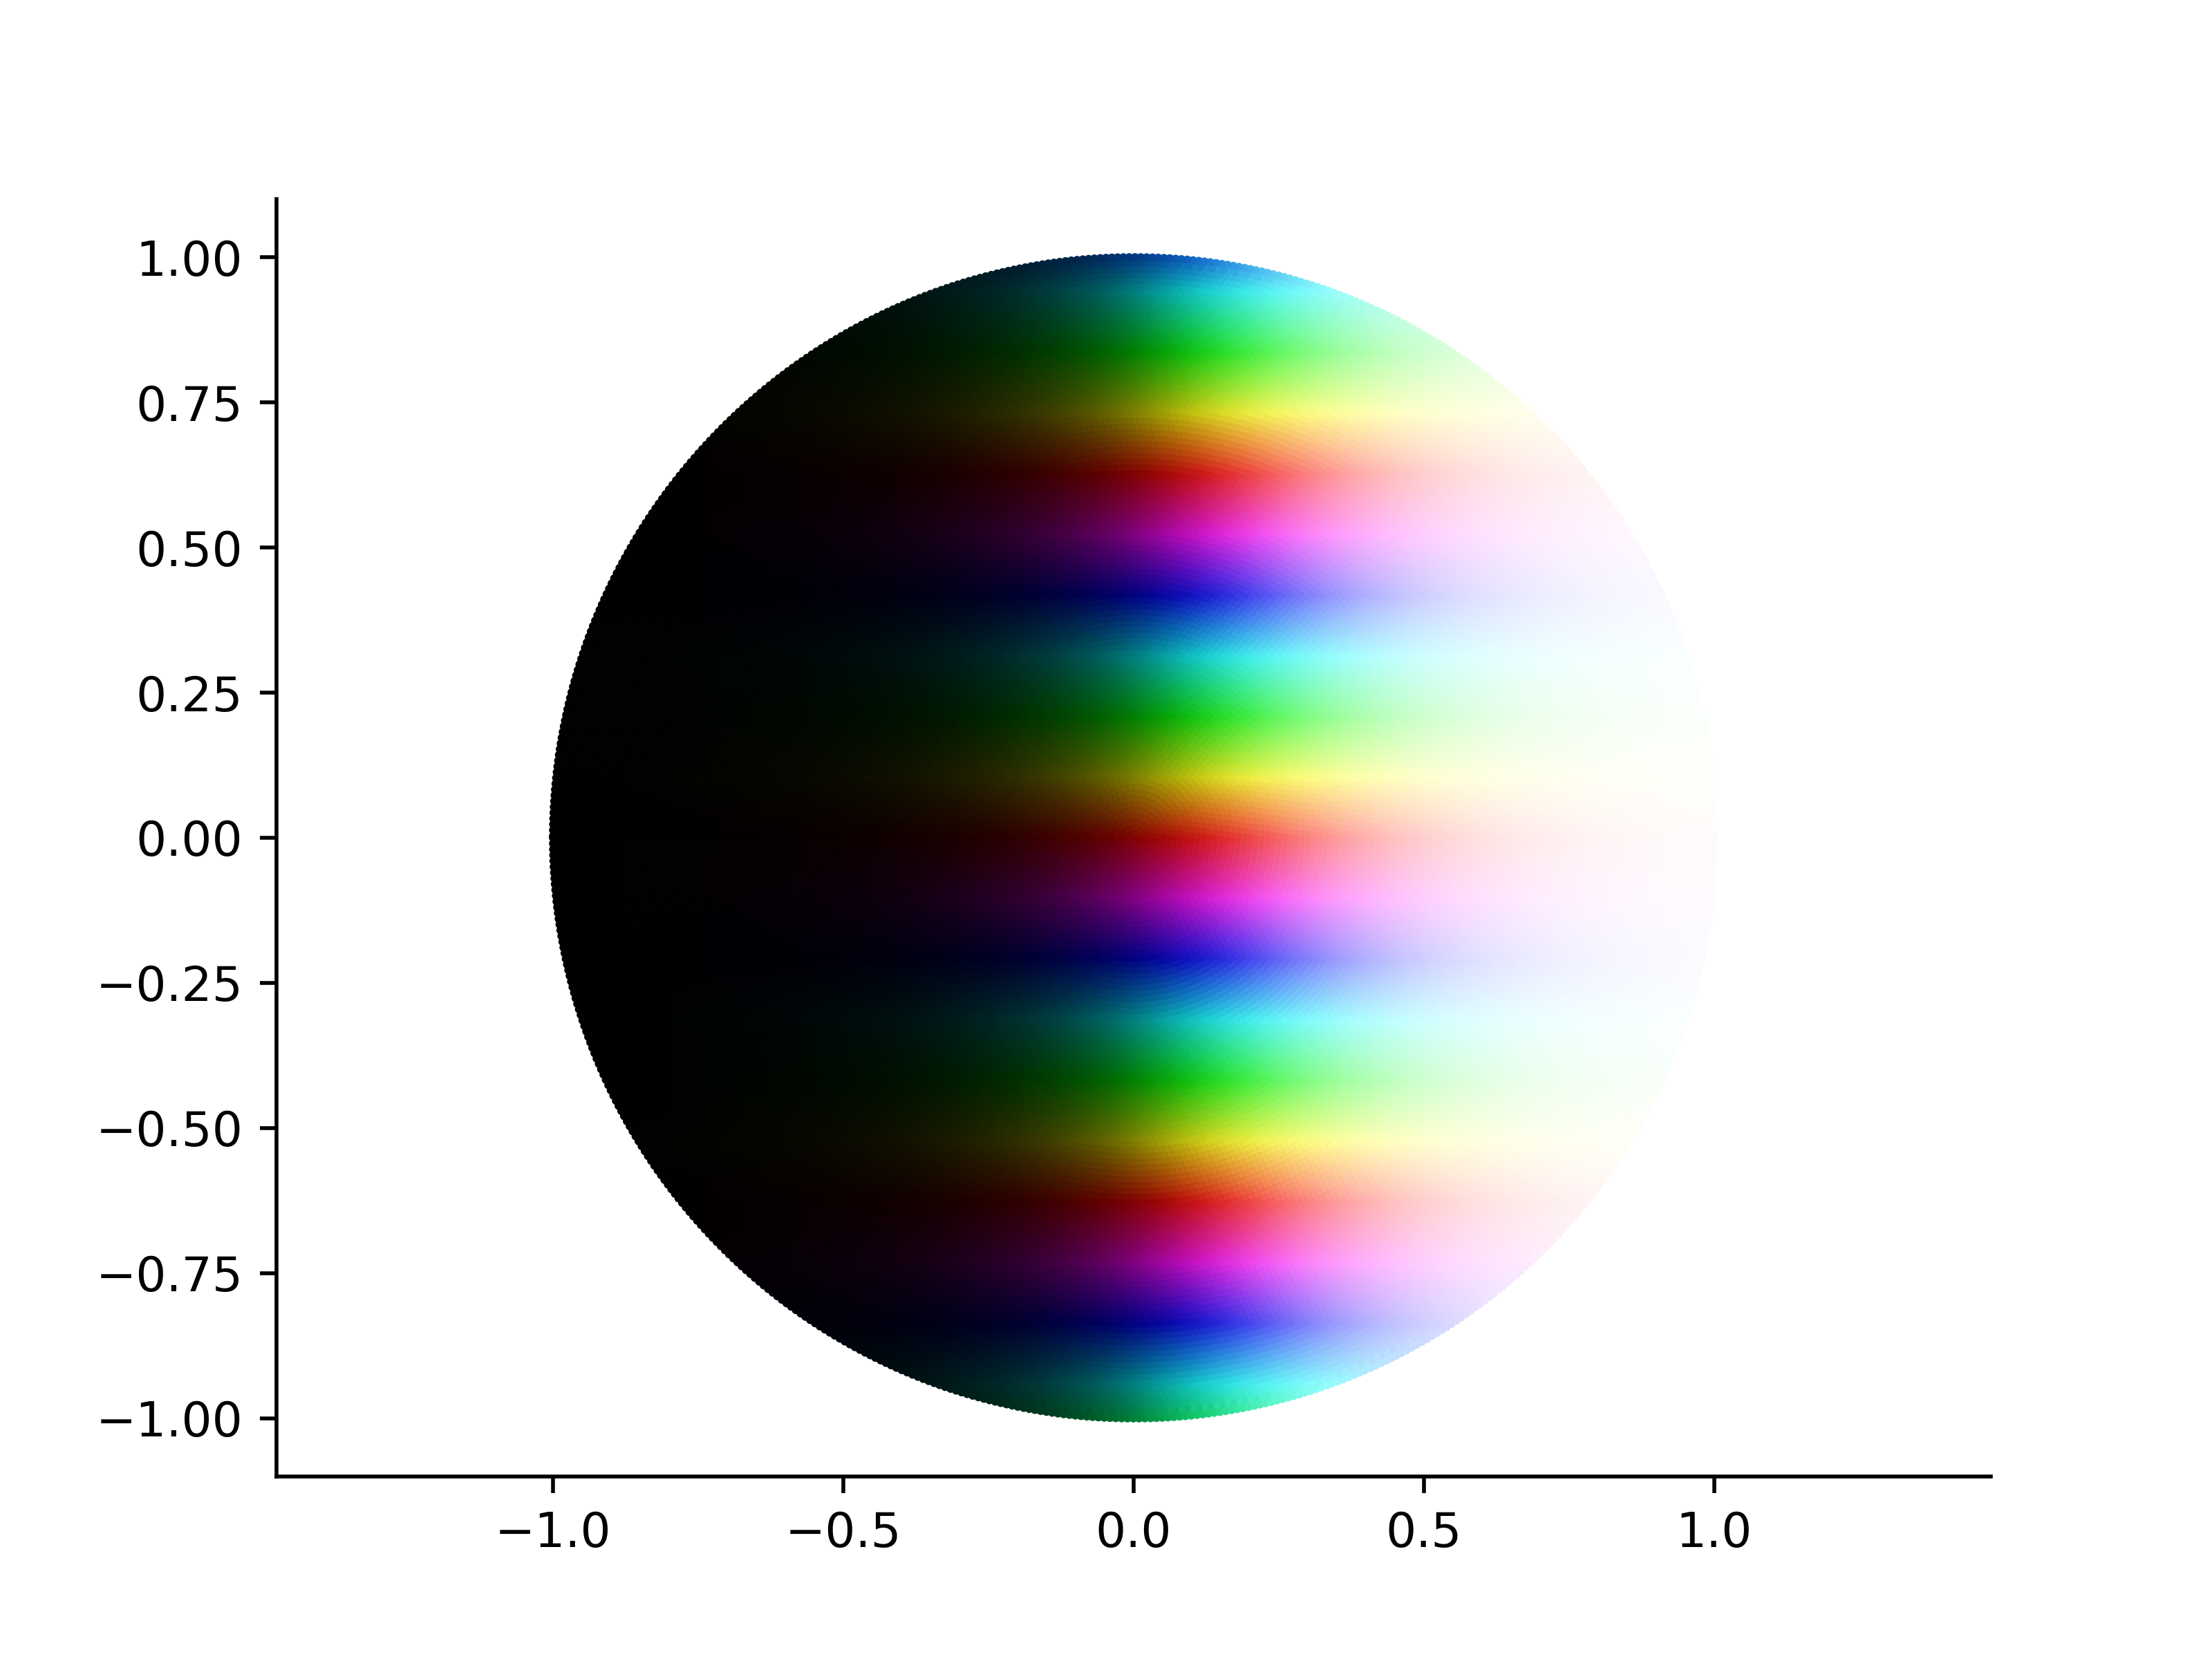
\includegraphics[width=0.7\textwidth]{../Aplicacion/e^(10cos(t)+10isen(t)).png}
        \label{fig:comp_e^z}
    \end{figure}
\end{frame}

\begin{frame}
    \frametitle{Extensión al disco de funciones con alguna discontinuidad en el borde}
    \begin{figure}[!htbp]
        \centering
        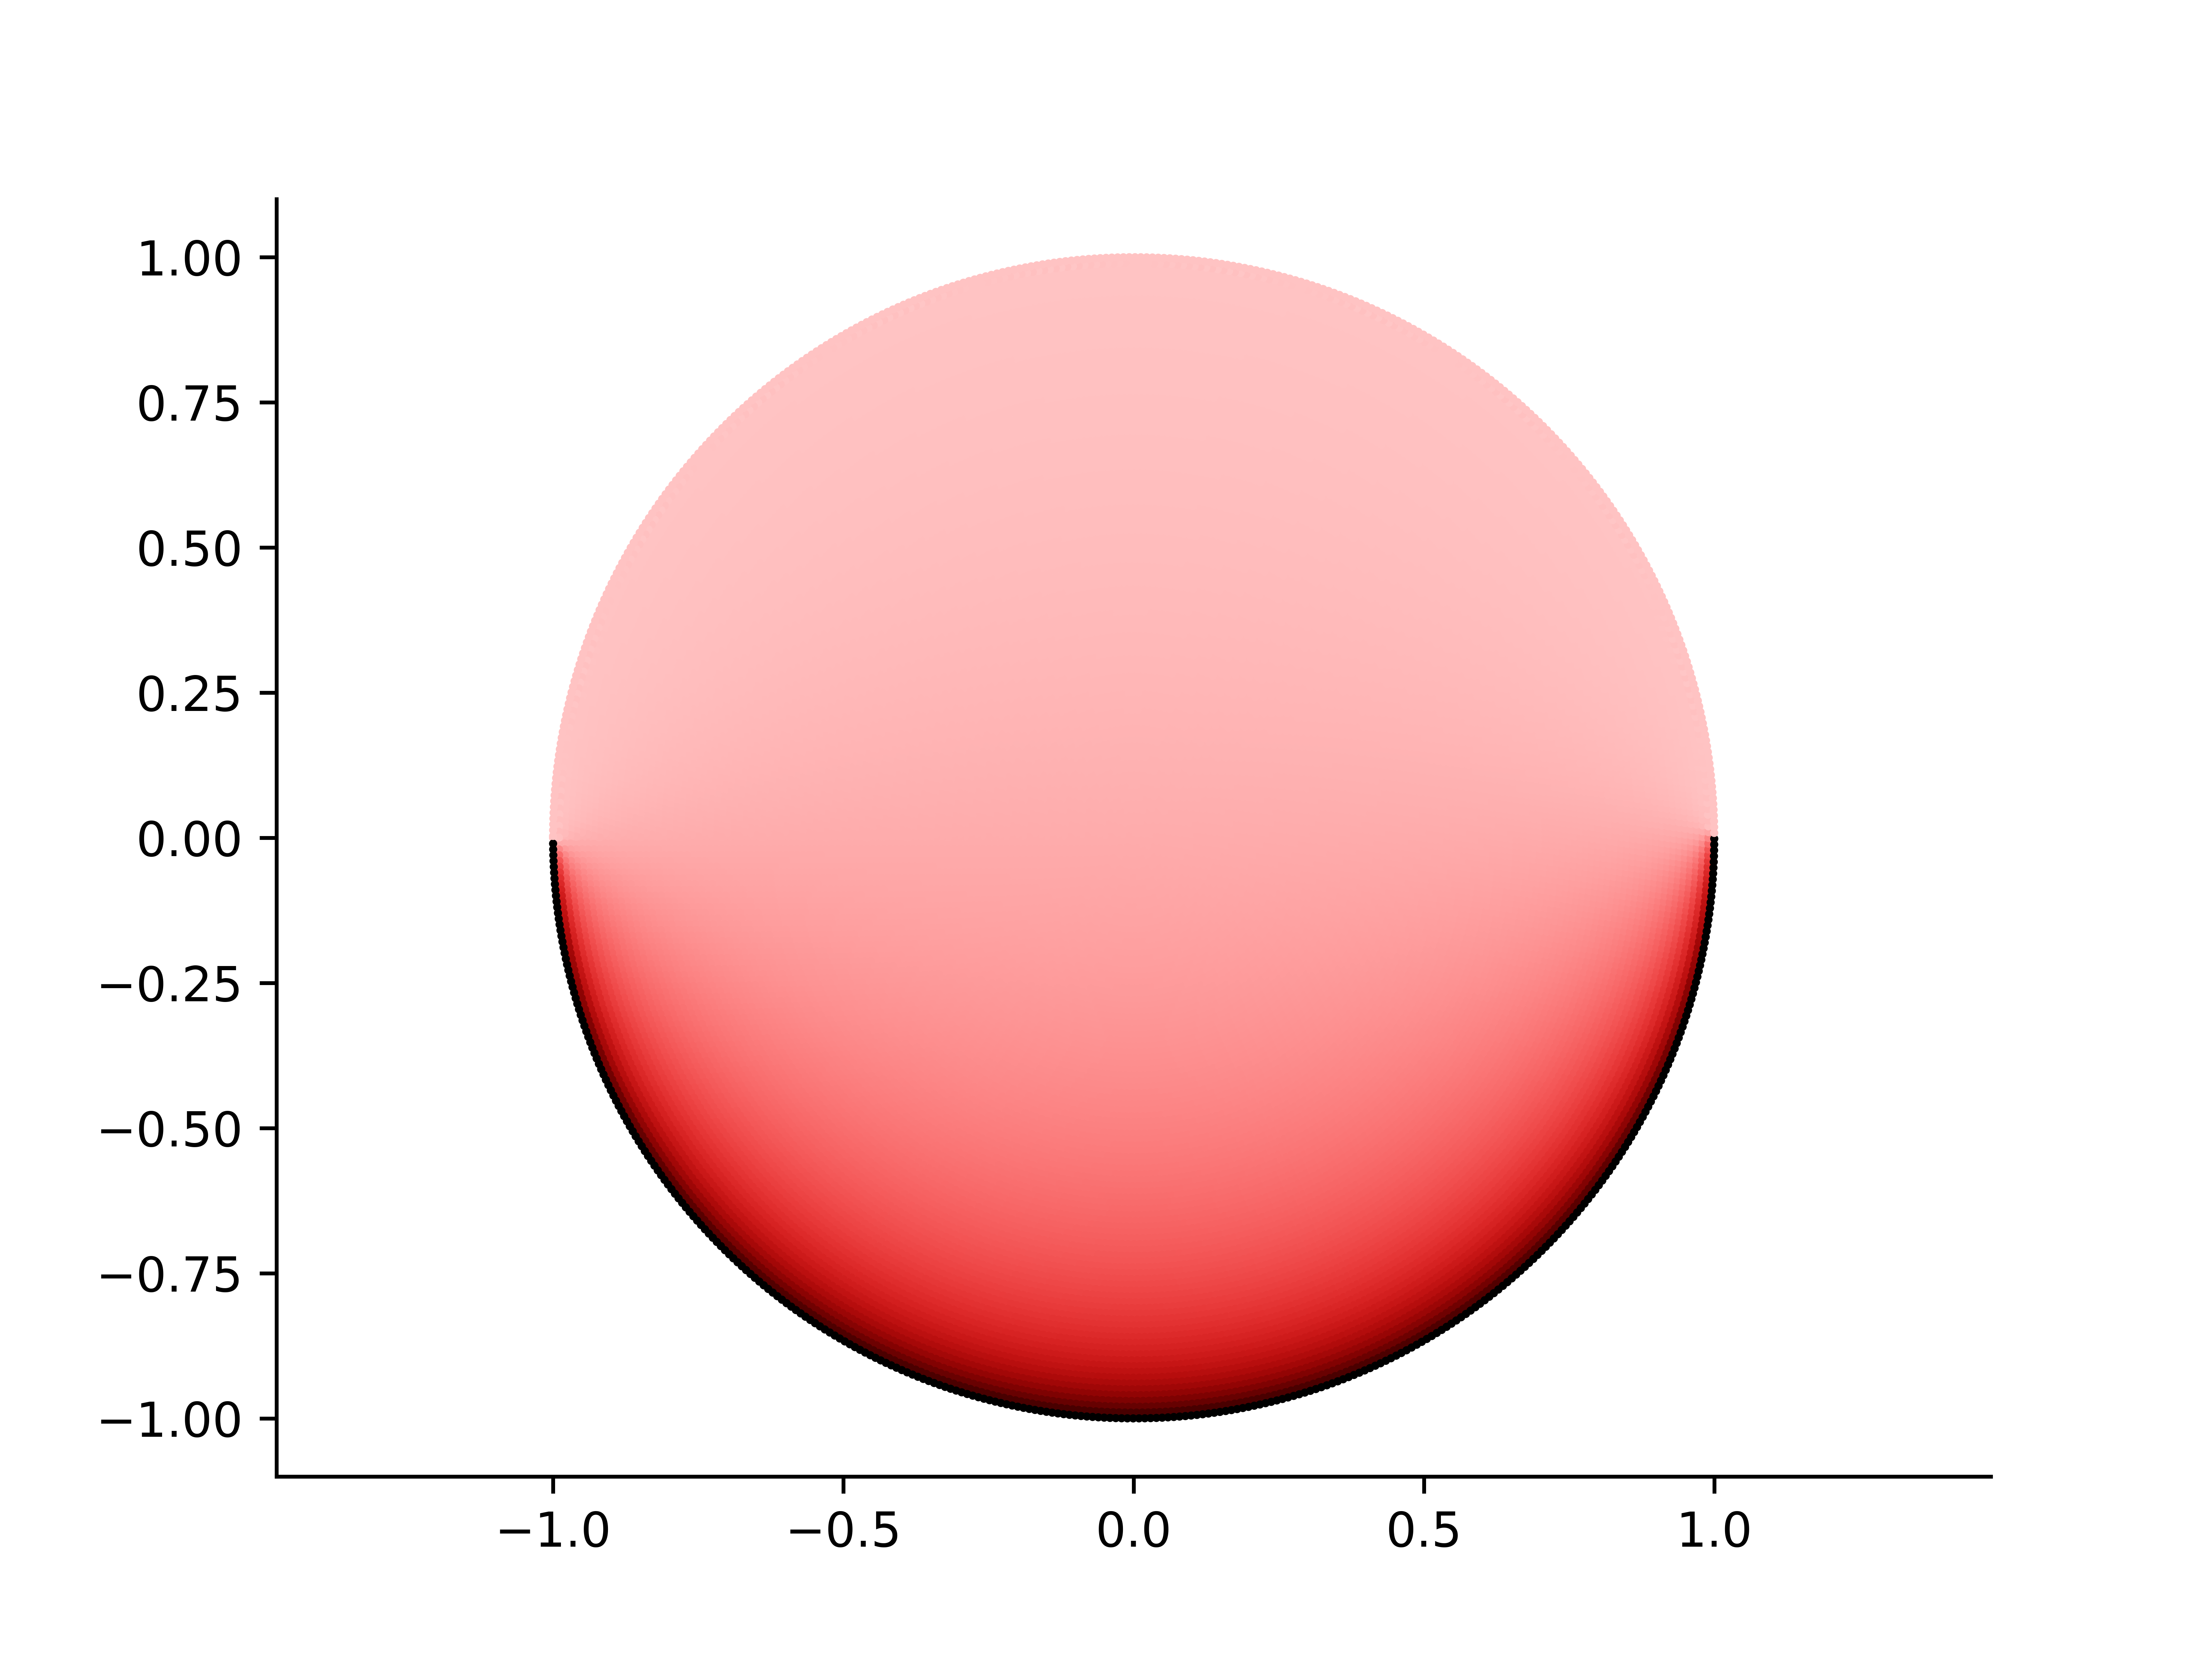
\includegraphics[width=0.49\textwidth]{../Aplicacion/atrozos.png}
        \hfil
        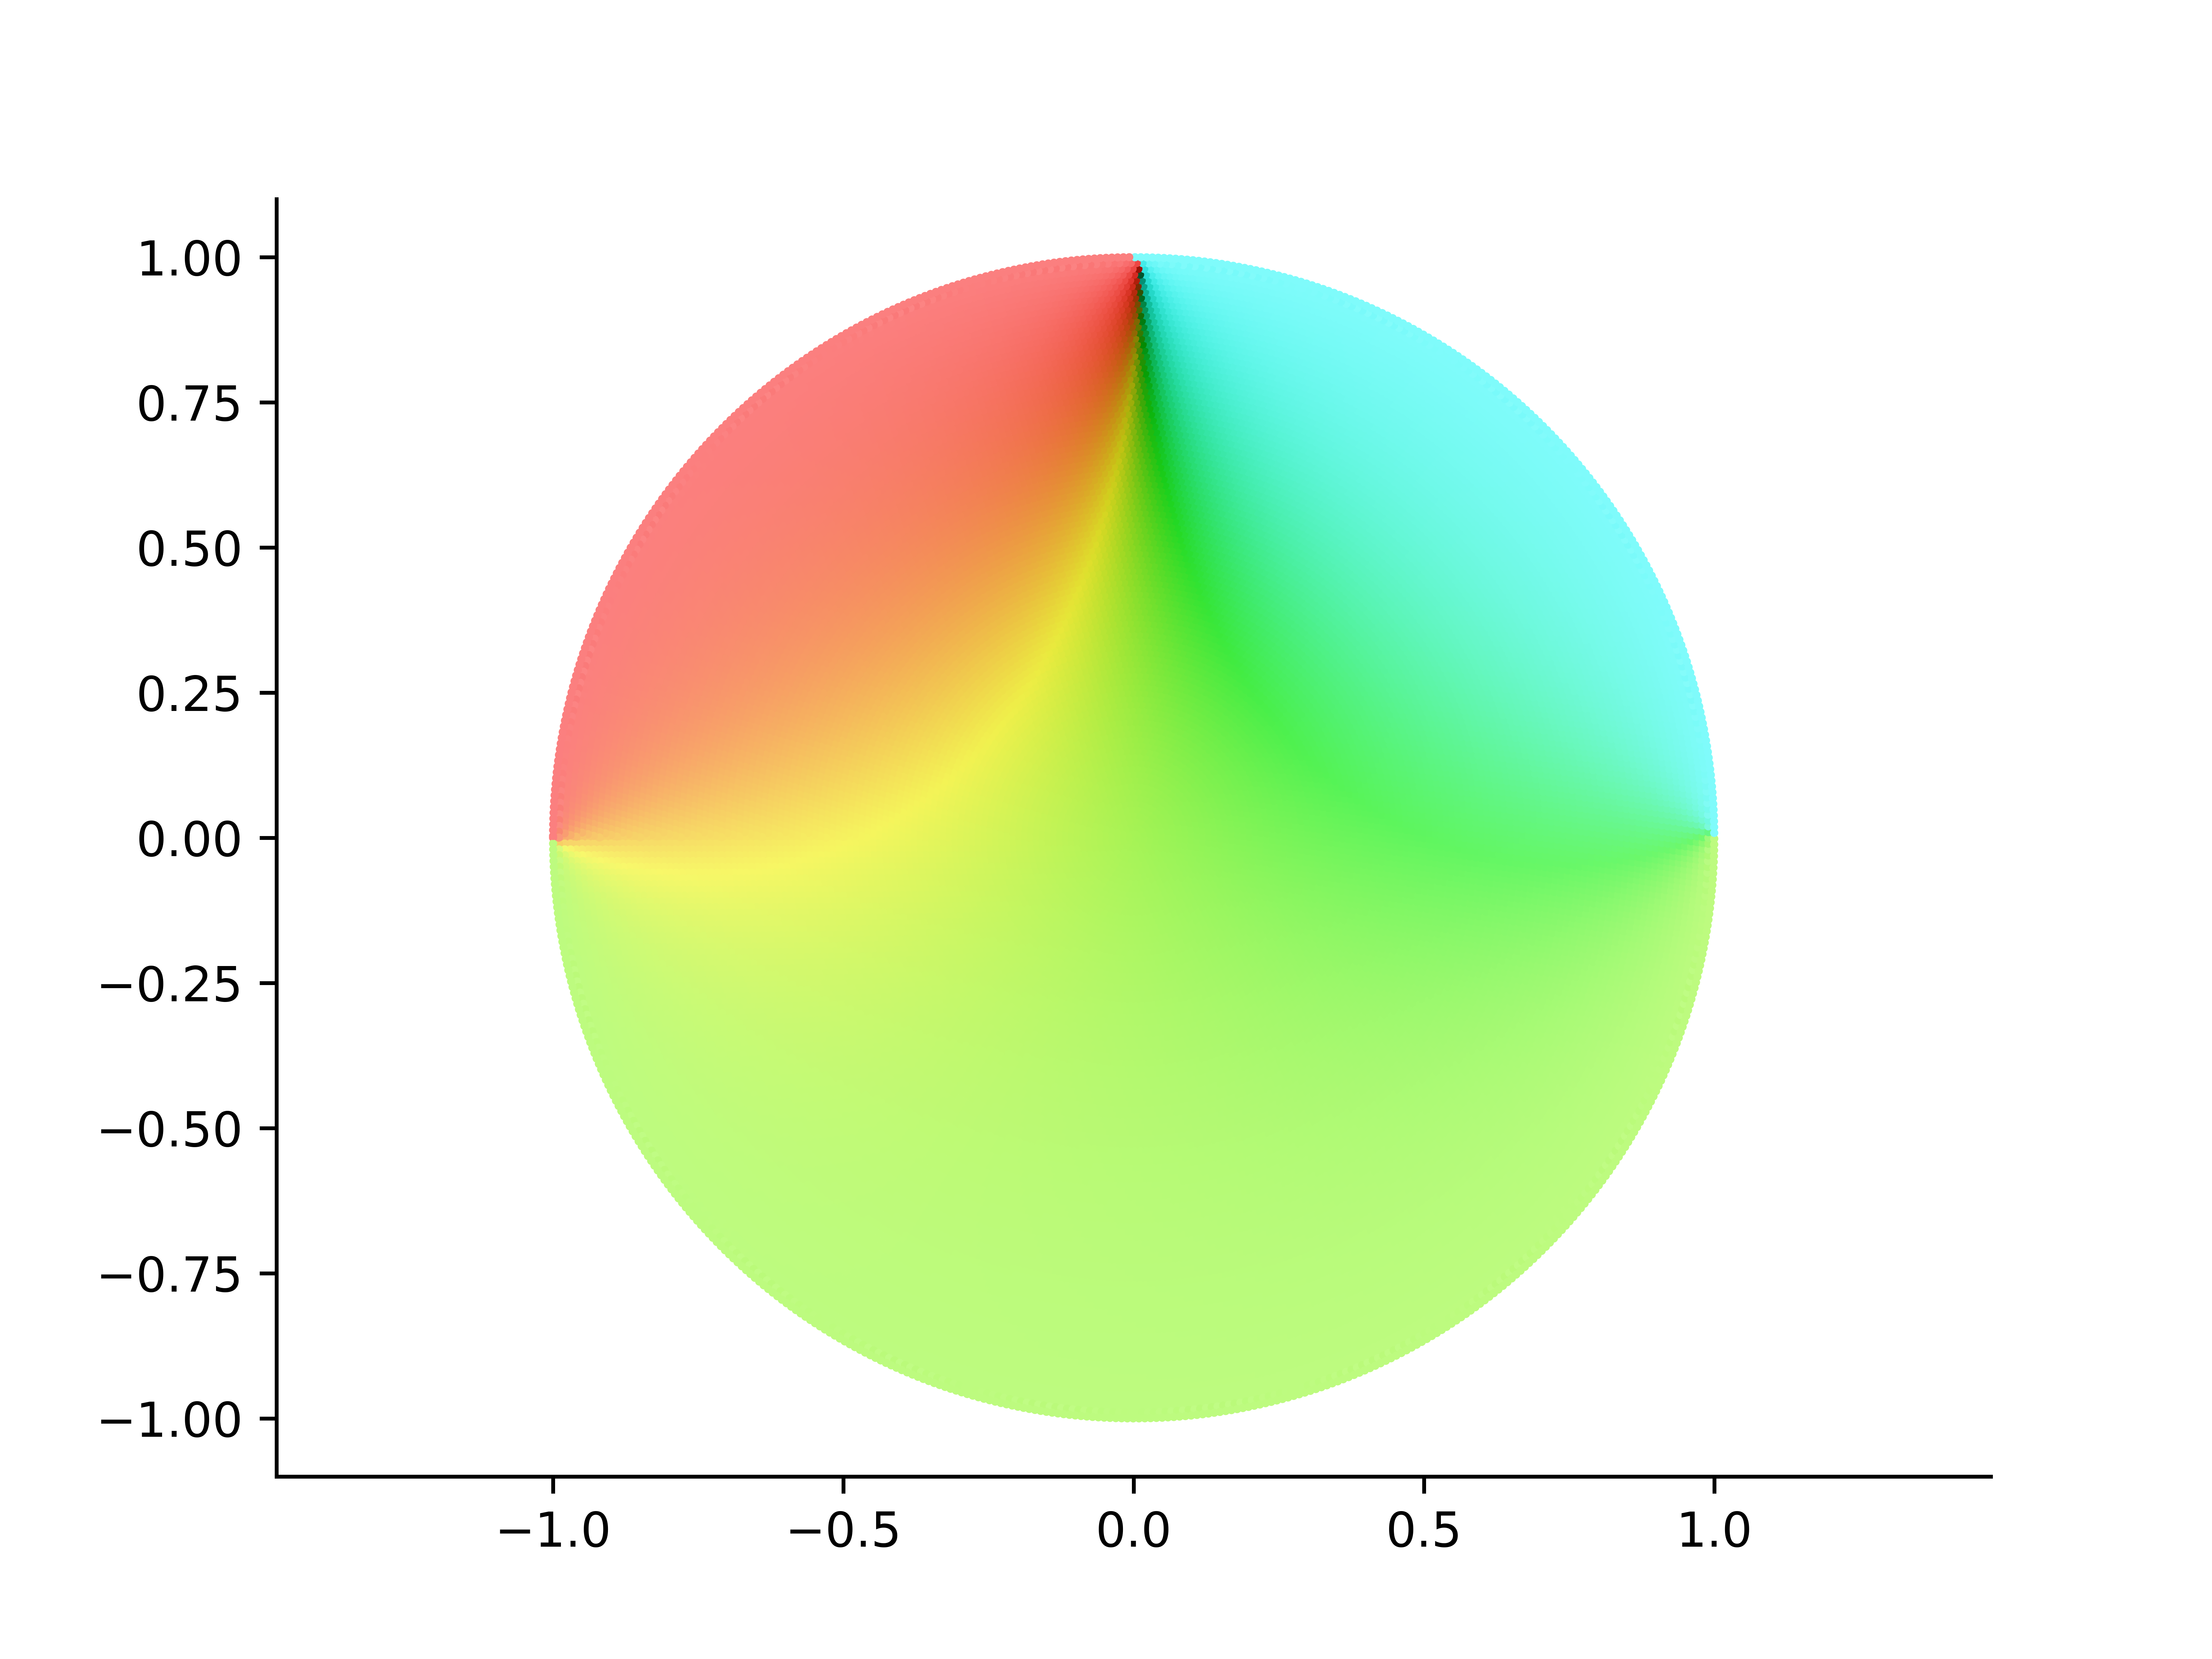
\includegraphics[width=0.49\textwidth]{../Aplicacion/atrozos(2).png}
        \label{fig:atrozos}
    \end{figure}
\end{frame}

\begin{frame}
    \frametitle{Código: color}
    \lstinputlisting[language=Python, firstline=39, lastline=55]{../Aplicacion/plotter.py}
\end{frame}

\begin{frame}
    \frametitle{Código: integral de Poisson}
    \lstinputlisting[language=Python, firstline=9, lastline=18]{../Aplicacion/function.py}
\end{frame}

\begin{frame}
    \frametitle{Código: integral de Poisson}
    \lstinputlisting[language=Python, firstline=20, lastline=36]{../Aplicacion/function.py}
\end{frame}

\begin{frame}
    \frametitle{Conceptos sobre álgebras de Banach}
    \begin{itemize}
        \item Un espacio vectorial complejo $X$, dotado de una norma $\norm{\cdot}$ se denomina espacio de Banach si es completo.

        \item Decimos que un álgebra $B$, dotada de una norma $\norm{\cdot}$ es un álgebra de Banach si como espacio normado $(B, \norm{\cdot})$ es un espacio de Banach y, además, para el producto satisface:
            \begin{equation*}
                \forall x, y \in B: \, \norm{x \cdot y} \leq \norm{x} \cdot \norm{y}.
            \end{equation*}

        \item $(\bholomorphic{\disk}, \norminf{\cdot})$ es un álgebra de Banach conmutativa.
    \end{itemize}
\end{frame}

\begin{frame}
    \frametitle{Espectro de $\bholomorphic{\disk}$ y transformada de Gelfand}
    \begin{itemize}
        \item El espacio dual de $\bholomorphic{\disk}$, denotado por $\bholomorphic{\disk}^*$, es el espacio de las aplicaciones $\phi: \bholomorphic{\disk} \to \complex$ lineales y continuas, cuya norma natural viene dada por:
            \begin{equation*}
                \norm{\phi} = \sup_{\norm{z} \leq 1} \abs{\phi(z)}.
            \end{equation*}

        \item El espectro de $\bholomorphic{\disk}$, denotado por $\fiber = \fiber (\bholomorphic{\disk})$, es el espacio de los homomorfismos $\phi: \bholomorphic{\disk} \to \complex$ no nulos.

        \item Transformada de Gelfand: $f \mapsto \widehat f$, con
            \begin{equation*}
                \begin{split}
                    \widehat f:  \fiber  & \to  \complex \\
                                 \phi \, & \mapsto  \phi (f),
                \end{split}
            \end{equation*}
    \end{itemize}
\end{frame}

\begin{frame}
    \frametitle{Fibras}
    \begin{itemize}
        \item Si $\alpha \in \closedisk$, la fibra de $\fiber$ sobre $\alpha$ se define como
        \begin{equation*}
            \fiber_\alpha = \{\phi \in \fiber : \phi (\id) = \alpha\}.
        \end{equation*}
    \end{itemize}

    \begin{block}{}
        Sea $f$ una función en $\bholomorphic{\disk}$ y sea $\alpha$ un punto del círculo unidad. Sea $\{z_n\}$ una sucesión de puntos en el disco unidad $\disk$ que converge a $\alpha$, y supongamos que el límite $\zeta = \lim_{n \to \infty} f(z_n)$ existe. Entonces existe un homomorfismo complejo $\phi$ en la fibra $\fiber_\alpha$ tal que $\phi(f) = \zeta$.
    \end{block}

    \begin{block}{}
        Sea $f \in \bholomorphic{\disk}$ y sea $\alpha \in \partial \disk$. La función $\widehat f$ es constante en la fibra $\fiber_\alpha$ si y solo si $f$ se puede extender con continuidad a $\disk \cup \{\alpha\}.$
    \end{block}
\end{frame}

\begin{frame}
    \frametitle{El conjunto de valores adherentes}
    \begin{itemize}
        \item  Dados $f \in \bholomorphic{\disk}$ y $\alpha \in \closedisk$, definimos el conjunto de valores adherentes de $f$ en $\alpha$ como
            \begin{equation*}
                Cl(f, \alpha) = \{\zeta : \exists \{z_n\} \subset \disk, \lim_{n \to \infty} z_n = \alpha, \lim_{n \to \infty} f(z_n) = \zeta \}.
            \end{equation*}

        \item El conjunto de valores adherentes de $f$ en $\alpha$ contiene un único punto si y solo si $f$ es continua en $\disk \cup \{\alpha\}$.
    \end{itemize}

    \begin{block}{} \centering
         $Cl(f, \alpha) = \widehat{f}(\fiber_\alpha)$.
    \end{block}
\end{frame}

\begin{frame}
    \frametitle{Representación de $e^{\frac{z+1}{z-1}}$}
    \begin{figure}[!htbp]
        \centering
        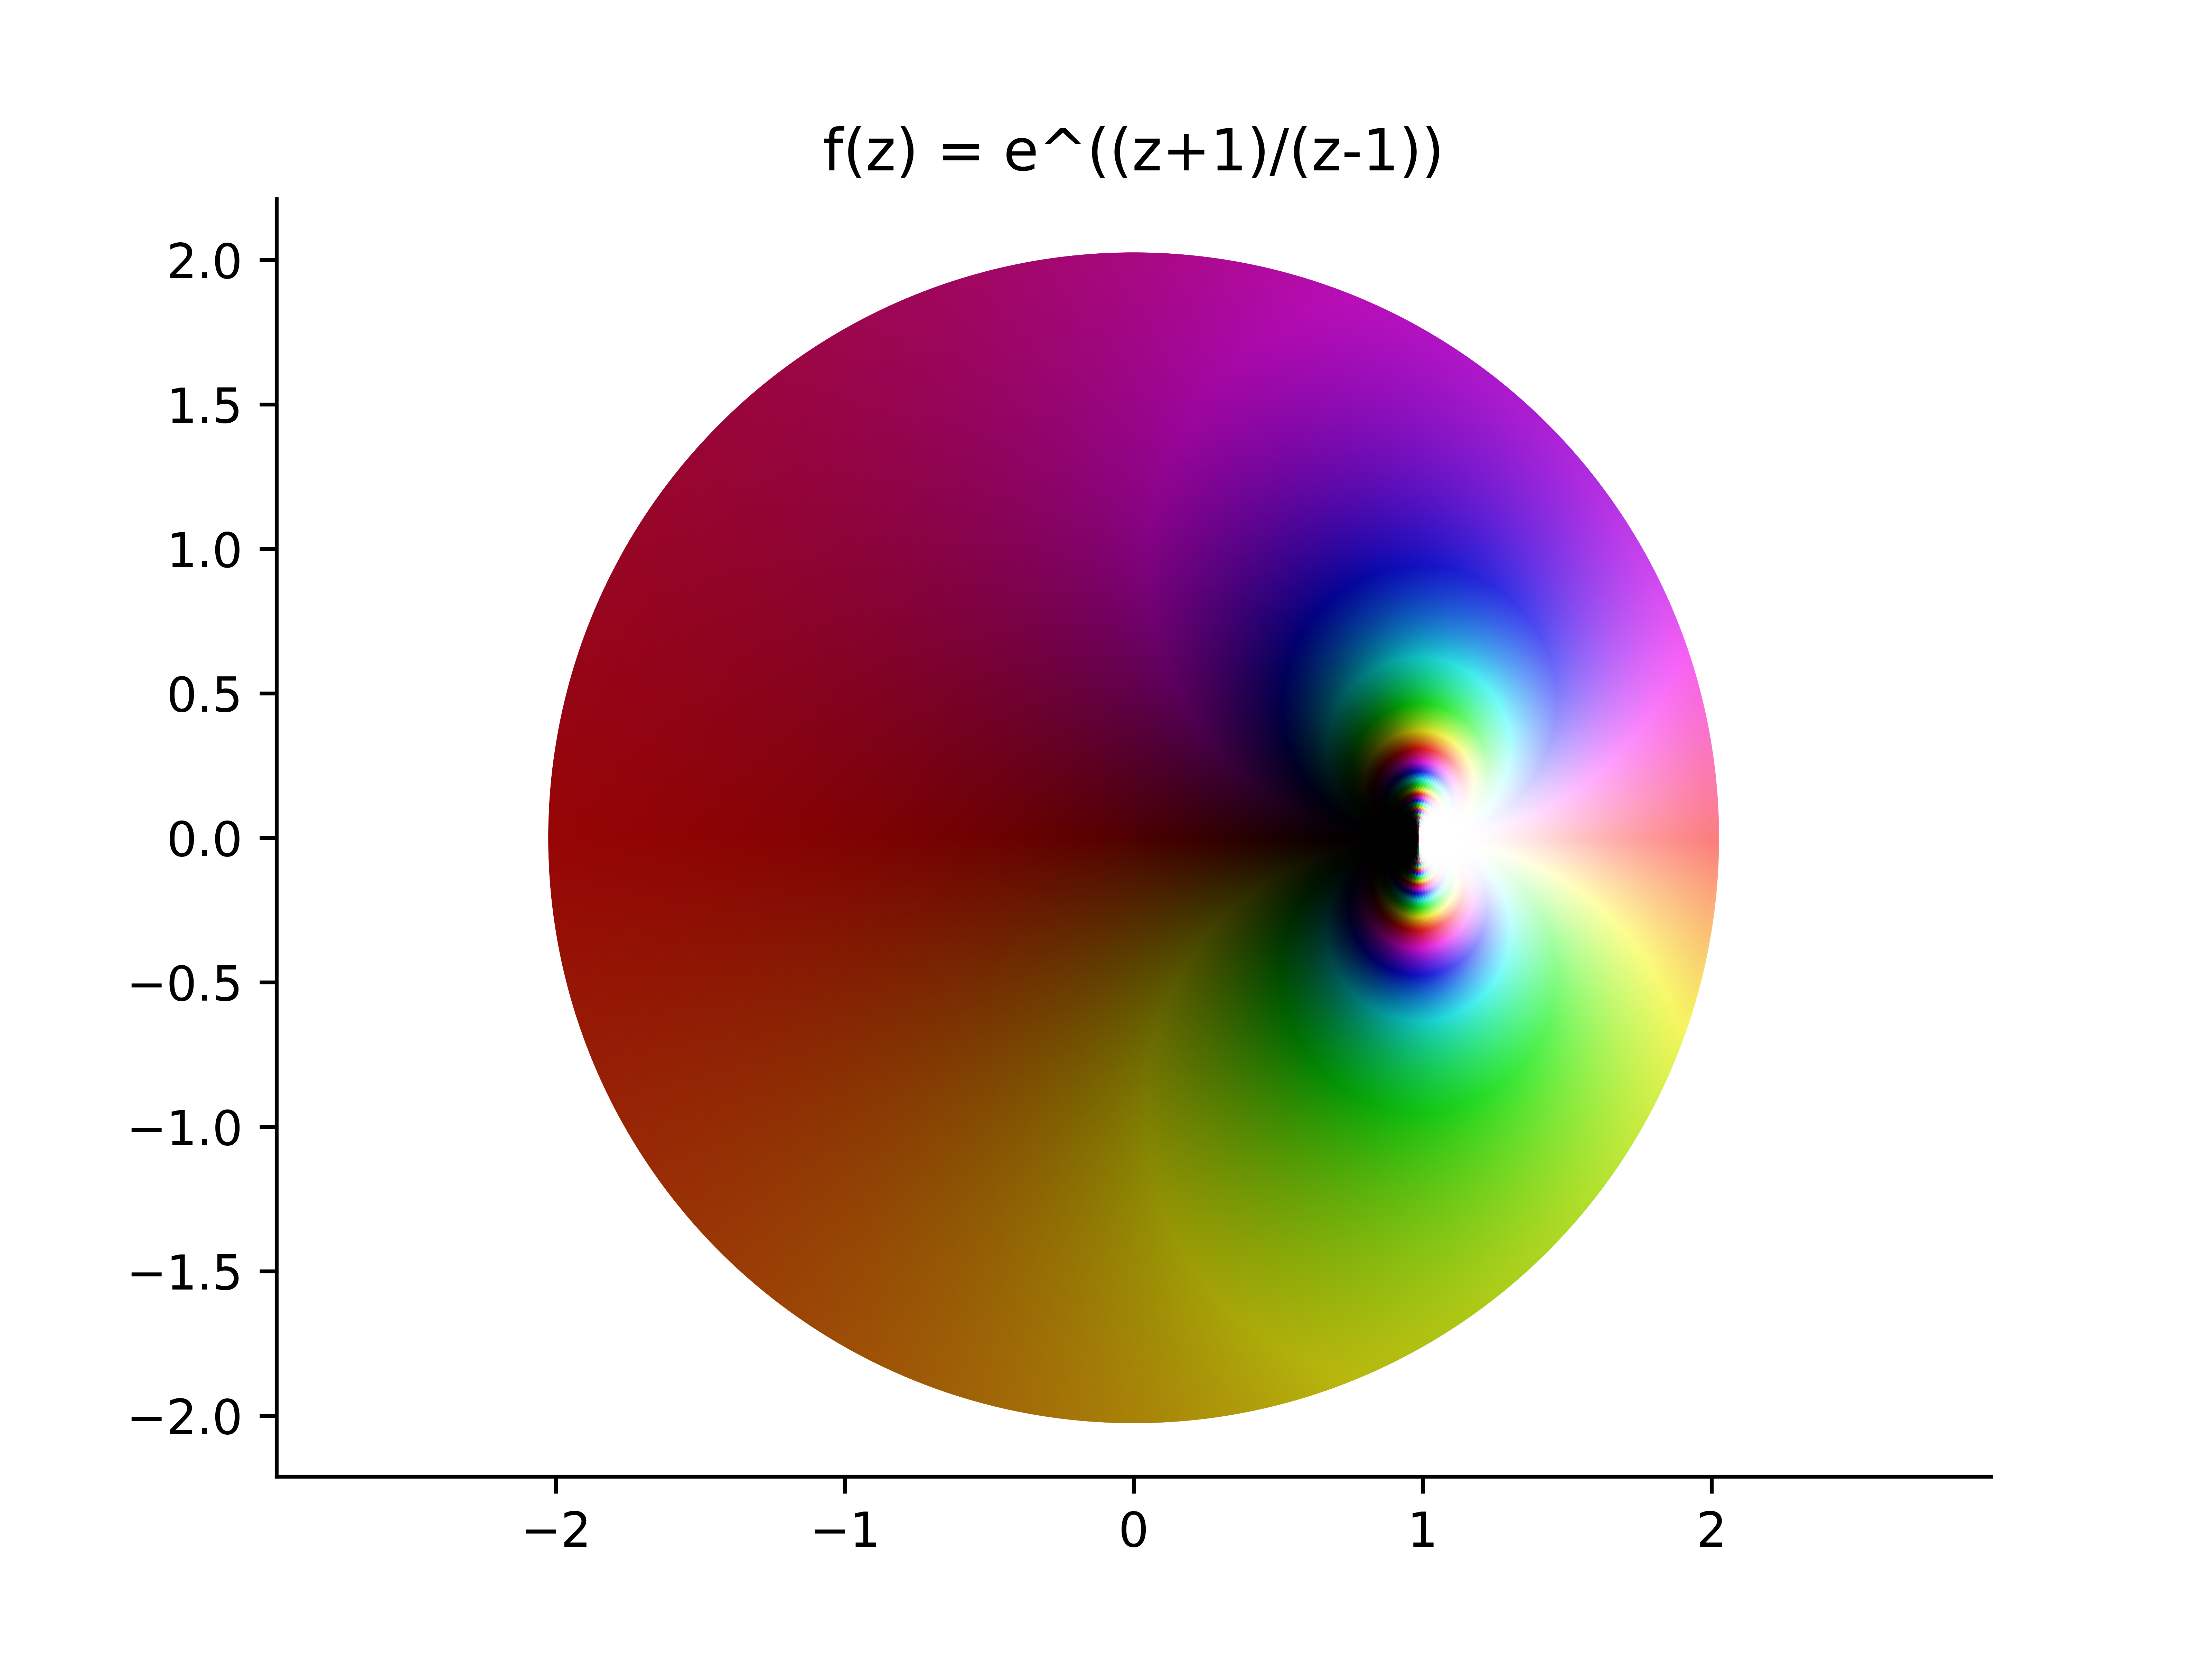
\includegraphics[width=0.7\textwidth]{../Aplicacion/e^((z+1):(z-1)).png}
        \label{fig:e^((z+1)/(z-1))}
    \end{figure}
\end{frame}

\begin{frame}
    \frametitle{Lema de Schwarz-Pick}
    \begin{itemize}
        \item Definimos la familia de automorfismos $\{\alpha_p: p\in \disk\}$ dada por
            \begin{equation*}
                \alpha_p (z) = \frac{p-z}{1 - \bar{p}z}, z \in \disk.
            \end{equation*}

        \item Definimos el disco no euclídeo de centro $p$ y radio $r$ como
            \begin{equation*}
                \Delta(p,r) = \left\{z \in \disk: \abs{\frac{p-z}{1 - \xbar{p}z}} < r\right\} = \left\{z \in \disk: \abs{\alpha_p(z)} < r \right\}.
            \end{equation*}

    \end{itemize}

    \begin{block}{Lema de Schwarz-Pick}
        Toda función holomorfa $f$ del disco $\disk$ en sí mismo lleva $\Delta(p,r)$ en $\Delta(f(p),r)$.
    \end{block}
\end{frame}

\begin{frame}
    \frametitle{Horodiscos}
    \begin{itemize}
        \item Llamaremos horodisco en el punto $w$ y radio $\lambda$ al conjunto
            \begin{equation*}
                H(w,\lambda) = \{z \in \disk : \abs{1 - \xbar{w} z}^2 < \lambda(1 - \abs{z}^2)\}.
            \end{equation*}
        \item Discos no euclídeos $\Delta(0, r)$, $\Delta(p_n, r_n)$ y horodisco $H(w, \lambda)$.
    \end{itemize}

    \begin{figure}[!htbp]
        \begin{minipage}[h]{0.35\textwidth}
            \centering
            \begin{tikzpicture}[scale=0.35]
                \draw (0, 0) circle (5cm);
                \draw[fill=lavander] (0, 0) circle (3.6cm);
                \filldraw[black] (0, 0) circle (2.0pt) node[below, font=\footnotesize] {$O$};
            \end{tikzpicture}
            \label{fig:noeuclideo1}
        \end{minipage} \hfill
        \begin{minipage}[h]{0.3\textwidth}
            \begin{tikzpicture}[scale=0.35]
                \draw (0, 0) circle (5cm);
                \draw[fill=lavander] (0.84,3.24) circle (1.1407015385279355cm);
                \filldraw[black] (0.8, 3.74) circle (2.5pt);
                \draw[color=black] (0.94, 4.11);
            \end{tikzpicture}
            \label{fig:noeuclideo2}
        \end{minipage} \hfill
        \begin{minipage}[h]{0.3\textwidth}
            \begin{tikzpicture}[scale=0.35]
                \draw (0, 0) circle (5cm);
                \draw[fill=lavander] (2.299024850013829,3.0883087788941905) circle (1.1500204535309522cm);
                \filldraw[black] (3, 4) circle (2.5pt);
            \end{tikzpicture}
            \label{fig:noeuclideo3}
        \end{minipage}
        \label{fig:noeuclideos}
    \end{figure}
\end{frame}

\begin{frame}
    \frametitle{Límite y derivada angular}
    \begin{itemize}
        \item Si $f$ es una función definida en $\disk$ y $w \in \partial \disk$, se define el límite angular de $f$ en $w$ como
            \begin{equation*}
                \angle \lim_{z \to w} f(z) = L.
            \end{equation*}

        \item Decimos que una función $f$ holomorfa del disco $\disk$ en sí mismo tiene derivada angular en $w \in \partial \disk$ si para algún $\eta \in \partial \disk$, el límite
            \begin{equation*}
                \angle \lim_{z \to w} \frac{\eta - f(z)}{w - z}
            \end{equation*}
            existe. Se dice que dicho límite es la derivada angular de $f$ en $w$ y lo denotamos por $\angle f'(w)$.
    \end{itemize}
\end{frame}

\begin{frame}
    \frametitle{Teorema de Julia}
    \begin{block}{}
        Si $f$ es una función holomorfa del disco $\disk$ en sí mismo no constante, y existen $w, \mu \in \partial \disk$ y una sucesión $\{p_n\} \in \disk$ que verifican
        {
        \leqnomode
        \setcounter{align}{0}
        \renewcommand{\thealign}{\alph{align}}
        \begin{align}
            & \lim_{n \to \infty} p_n = w;
            \alignno \\
            & \lim_{n \to \infty} f(p_n) = \mu;
            \alignno \\
            & \lim_{n \to \infty} \frac{1-\abs{f(p_n)}}{1-\abs{p_n}} = \delta < \infty.
            \alignno
        \end{align}
        }
        Entonces se cumple que
        {
        \leqnomode
        \setcounter{align}{0}
        \begin{align}
            & \delta > 0;
            \alignno \\
            & f(H(w, \lambda)) \subseteq H(\mu, \lambda \delta), \text{ para todo } \lambda > 0;
            \alignno \\
            & \angle \lim_{z \to w} f(z) = \mu.
            \alignno
        \end{align}
        }
    \end{block}
\end{frame}

\begin{frame}
    \frametitle{Representación de la función $g = \sigma^{-1} \circ \phi_a \circ \sigma$, con $a = \frac{1}{2}$.}
    \begin{figure}[!htbp]
        \centering
        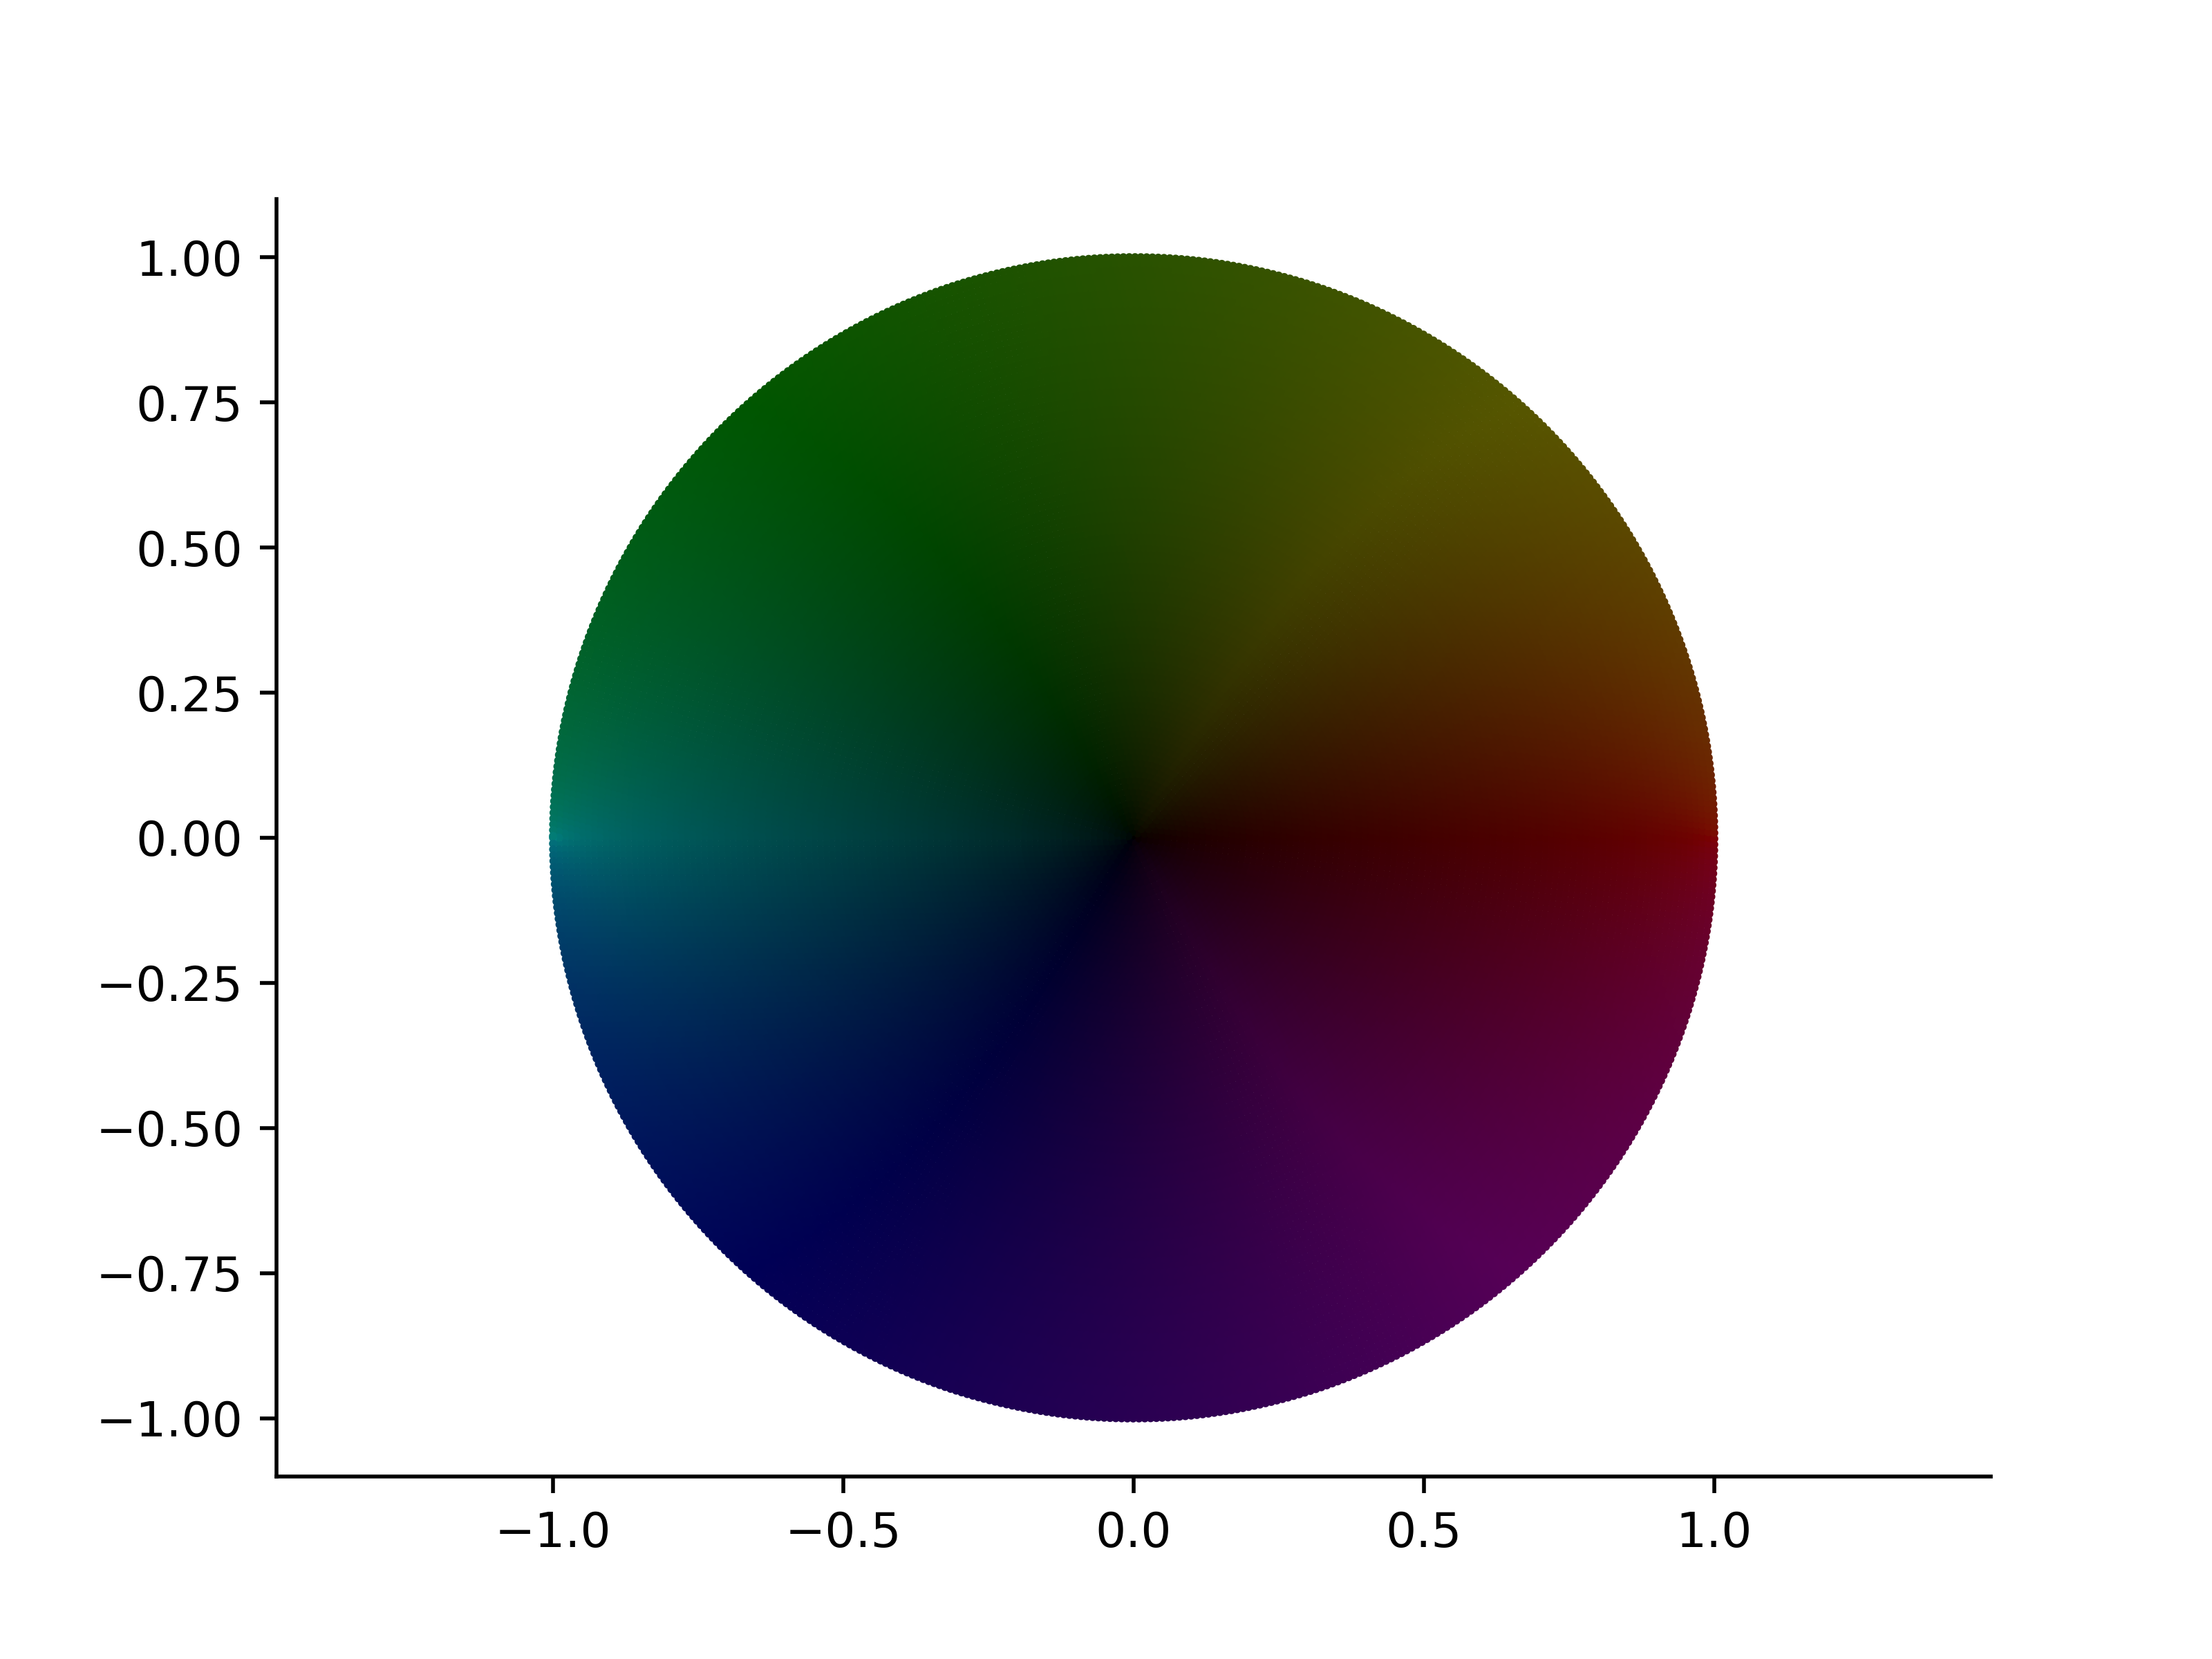
\includegraphics[width=0.7\textwidth]{../Aplicacion/lente.png}
        \label{fig:lente}
    \end{figure}
\end{frame}

\begin{frame}
    \frametitle{Bibliografía}
    \begin{itemize}
        \item \textit{Real and Complex Analysis} de Walter Rudin.
        \item \textit{Harmonic measure} de John B. Garnett y Donald E. Marshall.
        \item \textit{The Fundamental Theorem of Algebra: A Visual Approach} de Daniel J. Velleman.
        \item \textit{Banach Spaces of Analytic Functions} de Kenneth Hoffman.
        \item \textit{Composition Operators and Classical Function Theory} de Joel H. Shapiro.
    \end{itemize}
\end{frame}

\end{document}

